\documentclass[british,titlepage]{ntnuthesis}

\begin{figure}
\hspace{-2cm}
    \includegraphics[scale=.6]{figures/logo_ntnu_eng.png}
\end{figure}


\title{\LARGE \textbf{A novel hybrid flow cytometric approach to the Mussel micronucleus cytome assay}}
\author{Tørris Sandsæter}
\date{\today}

\shorttitle{ENVITOX Thesis}
\shortauthor{T. Sandsæter}

\addbibresource{nonauto.bib}



% From https://www.overleaf.com/learn/latex/Glossaries

\makeglossaries 

% --------------------
% ----- Acronyms -----
% --------------------

\newacronym{CoPCSE}{CoPCSE@NTNU}{Community of Practice in Computer ScienceEducation at NTNU}
\newacronym{ethd-1}{EthD-1}{Ethidium Homodimer-1}
\newacronym{fcm}{FCM}{Flow Cytometry}
\newacronym{fsc}{FSC}{Forward Scatter}
\newacronym{ssc}{SSC}{Side Scatter}
\newacronym{edta}{EDTA}{Ethylenediaminetetraacetic acid}
\newacronym{acb}{ACB}{Anticoagulant Buffer}
\newacronym{mas}{MAS}{Modified Alserver's Solution}
\newacronym{namas}{naMAS}{non-adjusted Modified Alsever's Solution (pH = 6.1)}
\newacronym{mpss}{MPSS}{Marine Physiological Saline Solution}
\newacronym{fsw}{FSW}{Filtered Seawater}
\newacronym{wwtp}{WWTPs}{Waste-Water Treatment Plants}
\newacronym{ENPs}{ENPs}{Engineered Nano Particles}
\newacronym{tbs}{TBS}{Tris-Buffered Saline}
\newacronym{glmms}{GLMMs}{Generalized Linear Mixed Models}
\newacronym{Ag}{Ag}{Silver}
\newacronym{tio2}{\ce{TiO2}}{Titanium(IV)oxide}
\newacronym{dmso}{DMSO}{Dimethyl Sulfoxide}
\newacronym{dsdna}{dsDNA}{Double-Stranded DNA}
\newacronym{calceinam}{Calcein AM}{Calcein AcetoxyMethyl}
\newacronym{apo15}{Apo-15}{BioTracker Apo-15 Calcium-independent Apoptosis Probe}
\newacronym{emmax}{Em$_{max}$}{Emission Maximum}
\newacronym{exmax}{Ex$_{max}$}{Excitation Maximum}
\newacronym{meoh}{\ce{MeOH}}{Methanol}
\newacronym{mfi}{MFI}{Mean Fluorescent Intensity (arbitrary units)}
\newacronym{fmo}{FMO}{Fluorescence Minus One (control)}
\newacronym{ps}{PS}{PhosphatidylSerine}
\newacronym{mae}{MAE}{Mean Absolute Error}
\newacronym{mni}{MNi}{Micronuclei}
\newacronym{mn}{MN}{Micronucleus}



\newacronym{mle}{MLE}{Maximum Likelihood Estimate}
\newacronym{fl1}{FL1}{Fluorescence detector 1 (533/15 nm)}
\newacronym{fl4}{FL4}{Fluorescence detector 4 (675/25 nm)}

\newacronym{thc}{THC}{Total Haemocyte Count}
%TP3 - TO-PRO-3 TM Iodide





 % add glossary and acronym lists before document

\begin{document}

\chapter*{Acknowledgments}
This master's thesis in Environmental Toxicology was conducted as a part of the ENTRANS project (302004820/NFR 302378?) at the Department of Climate and Environment, Sintef Ocean. Academic supervisor has been Senior Researcher Julia Farkas, Sintef Ocean and main supervisor Professor Bjørn Munro Jenssen, NTNU.

Include the full name of the project?, multi-disiplinary research project, funded by the Norwegian Research Council, led by NIVA, cooperation between NIVA, Sintef Ocean, etc.
Name of the project tox part that I'm involved with

Thanks to supervisors
Julia Farkas, Senior Research scientist, Sintef Ocean, Department of Climate and Environment
and
Prof. Bjørn Munro Jenssen, Institute of Biology, NTNU.

And thanks to staff at Sintef Ocean, Depratment of Climate and Environment:

Marianne Aas, Research Engineer,  Sintef Ocean, Department Climate and Environment.

Marianne Molid, Senior Engineer, Sintef Ocean, Department Climate and Environment.

Stefania Piarulli, Research scientist, Sintef Ocean, Department Climate and Environment.

NTNU

Dag Altin, Chief Engineer, NTNU.



\input{chapters/0b-abstract}
\input{chapters/0c-sammendrag}

\tableofcontents
\listoffigures
\listoftables


\printglossary[type=\acronymtype] % Print acronyms
\printglossary                    % Print glossary

\chapter{Introduction}
\section{The mussel micronucleus cytome Assay}
Micronuclei (\acrshort{mni}) are small cytosolic membrane-enclosed chromatin bodies that contain acentric chromosome fragments or whole lagging chromosomes that remain outside the nucleus of daughter cells after cell division (\cite{Fenech2011}). Micronuclei with acentric fragments can originate from unrepaired or misrepaired DNA-breaks from interactions with clastogenic chemicals, while larger MNi with whole chromosomes arise from indirect interactions with the replication apparatus during anaphase (aneugenic mechanism) (\cite{Fenech2011}). While the two structures may provide mechanistic information about the tested chemical, they are not readily distinguishable in standard cytologic preparations (\cite{Natarajan1993}). Without specific labeling of kinetochores or centromere-specific DNA, MNi provide general evidence for accumulated direct or indirect genotoxic damage during the cell life (\cite{Tucker1996, Lynch1993}).

These cytogenic damages are the major endpoints of micronucleus assays, which represent instrumental tests in the hazard identification of genotoxic compounds (\cite{OECD474, OECD487, USEPA1998}). Since there is a strong association between specific cytogenic alterations and tumorigenesis, the implementation of this biomarker in toxicological risk assessment is well justified (\cite{Mitelman1983} in: \cite{Tucker1996}). Micronucleus tests are performed on dividing or newly divided cells, and are most typically used to assay genotoxic damage in cells from bone marrow samples and blood in the case of mammalian test systems (\cite{Heddle1983, Warheit2018b}).

Micronucleus tests have also been extended for use in ecotoxicology, and represent one of the most prevalent biomarkers of genotoxicity in aquatic animals (\cite{Bolognesi2011}). Up to date, such eco-genotoxicity assays have most notably been performed in fish erythrocytes (reviewed in \cite{Agostini2021}) and in bivalve haemocytes and gill cells (reviewed in \cite{Bolognesi2014}). Bivalve mussels have gained a central role as sentinels in marine ecotoxicology studies, and the widespread blue mussel (\emph{Mytilus spp.}) has received a lot of attention in particular. Because of their limited biotransformation capacity (\cite{Beyer2017b}), low mortality (\cite{Ale2019, Costa2009}) and ability to accumulate a wide range of pollutants as filter-feeders; \emph{Mytilus spp.} has become the focal point of national monitoring programs of coastal water pollution (\cite{Goldberg1975, Beyer2017b, Cajarville2000}). In such programs (Mussel Watch Program), the micronucleus tests on caged mussels have been proposed as the only core biomarker of genotoxicity (\cite{Bolognesi2012}).

By following the cytome approach applied i mammalian systems (\cite{Fenech2007}), Bolognesi and Fenech (2012) updated and refined the existing MN test for bivalve haemocytes and gill cells to include scoring of necrotic and apoptotic cells as endpoints of cytotoxicity. Nuclear buds (\acrshort{nbuds}) were also included as a biomarker of elimination of amplified DNA and/or DNA repair complexes, although the mechanism leading to NBUD formation is not completely known (\cite{Bolognesi2012}). In addition to scoring cytogenic damage (MNi and NBUDs) and cytotoxic alterations (necrosis/apoptosis), a differential count of the agranular and granular haemocytes cell types were included in the protocol. As these innate immune cells have been found to exhibit different immunocompetences with regard to phagocytic activity, encapsulation and the secretion of cytotoxic molecules in host defence (\cite{delaBallina2022}), changes in the circulating haemocyte cell types may serve as indicators of stress and provide information on the immunological health status of mussels (\cite{Couch1993}).

Several contaminants have been shown to induce changes in the haemocyte profile of bivalves (\cite{Couch1993}). Among the tested contaminants, these include Cd$^{2+}$ and Cd-based quantum dots (\cite{Rocha2014, Auffret1994}), Cu$^{2+}$ (\cite{Pipe1995, Pipe1999}), Phenol (\cite{Fries1980}) and certain \acrshort{pahs} (\cite{Dyrynda1998, Dyrynda2000}). Since the mussel micronucleus cytome assay includes a differential haemocyte count in combination with two biomarkers of cytotoxic damage, an integrated interpretation of these endpoints might provide mechanistic information about the immunomodulating effects of potential cytotoxic chemicals. 

In spite the widespread adoption of the micronucleus cytome assay, this protocol has several limitations or drawbacks; most of which has the potential to be addressed by flow cytometry. First of all, the entire procedure is reported to take approximately 1 hour per individual mussel (\cite{Bolognesi2012}). If multiple sampling sites are employed with 10 individuals/site, the time required for a larger study soon reaches substantial proportions. Secondly, the added complexity of scoring cytotoxic alterations, genotoxic damages and performing differential counts in parallel might divert attention from the main endpoint. As MNi are rare events scored among a relatively small subset of cells (> 1000 agranular haemocytes), a few false negatives can potentially have a significant effect on the MNi frequencies of mussels from sites with low contaminant levels. The third limitation is related to the complexity of the haemocyte cell types, and the operator's subjective interpretations or classification of these and their cytotoxic alterations in the haemocyte preparations. 

The classification of bivalve haemocytes is a comprehensive literature that is dominated by a lack of scientific consensus (\cite{Hine1999}). For operators that rely on the images provided by the protocol for their practical classification, the first inspection of a haemolymph preparation may not paint a picture that is all that intuitive. Bolognesi and Fenech (2012) proposed scoring of MNi in agranular haemocytes, which were characterized by their small size (3-4 \micro m), high N:C ratio and lack or low abundance of cytoplasmic granules and organelles. As slight deviations from the staining protocol might produce striking differences in the overall staining result, the subjective interpretations of the observed cell types may produce large inter-operator variability in the scored cell population and the differential haemocyte count. This is highlighted by the fact that most operators fail to comment on the scored cell type (\cite{Bolognesi2012}), or erroneously score what they believe to be agranular haemocytes (e.g., \cite{Meng2020}). Since the granular haemocytes of \emph{M. galloprovincialis} are reportedly less sensitive to MN induction (\cite{Venier1997}), confusion of this sort can possibly reduce the sensitivity and inter-lab comparability of the micronucleus cytome assay. 

The difficulty of producing high quality preparations is another factor that might further complicate this issue. Haemolymph smears often have numerous staining artifacts and cells that are damaged during preparation. As a consequence, distinguishing cytotoxic alterations from staining artifacts may be challenging to operators without comprehensive training in histology or hematology. The identification of necrotic haemocytes based on extensive cytoplasmic vacuolation might be especially challenging in this context, as
both granular cell types of \emph{M. edulis} are phagocytic cells, and often display numerous phagosomes in their cytoplasm (\cite{Moore1977}). Damaged cell membranes - and the paler cytoplasmic staining that results from it - may also be hard to distinguish from irrelevant staining artifacts. 

In short, manual scoring of cytogenic damage in a defined cell population is a time-consuming and labor-intensive process with low throughput. The expanded scope of the micronucleus cytome assay further aggravates this fact, and a reference material consisting of a few PNG images leaves too much room for subjectivity in the identification of haemocyte cell types and cytotoxic alterations. As flow cytometers are permanent fixtures of cell biology labs these days, this high throughput cytologic instrument is availible to most ecotoxicologists involved in cellular work. With the capacity to differentiate single cells based on size, granularity and molecular markers, flow cytometry is a powerful tool for performing differential blood cells counts (\cite{Shapiro2004}), as well as scoring necrotic and apoptotic cells (\cite{Shapiro2003}). A hybrid flow cytometry/microscopy protocol of the micronucleus cytome assay has therefore great potential to improve the power and efficiency of the existing methodology, while creating less room for subjectivity.

\section{Classification of haemocyte subpopulations in \emph{M. edulis}}
\label{subsection:haemocyte_classification}
Since the first written account on the subject (\cite{Cuenot1891}, cited in: \cite{Cheng1980}), several authors have devoted their attentions to developing a unifying classification system for the amoebocytic blood cells of bivalve mollusks, more commonly known as haemocytes (\cite{Cheng1980, delaBallina2022}). The haemocytes of \emph{Mytilus edulis}, \emph{Mytilus galloprovincialis} and other commercially important species of the genus \emph{Mytilus} have been encompassed by these efforts, which has created a substantial pool of literature on the haemocytes of this genus alone. Despite a lack of consensus for any unifying classification system for the haemocytes of this phylum at large, the literature that exists on the haemocytes of \emph{M. edulis} generally agrees on the existence of three distinct subpopulations.

The first effort to classify the haemocytes of \emph{M. edulis} was made by Moore and Lowe (1977). Much like other attempts to classify bivalve haemocytes at the time, this classification was based on the morphofunctional aspects of these cells - a system that has been extensively reviewed by Hine (1999). Moore and Lowe constructed a simple classification based on static morphological and ultrastructural characteristics of the haemocytes, combined with their phagocytic capacities (\cite{Moore1977}). From routine cytological staining, they identified three haemocyte subpopulations (or cell types): "(1) small basophilic hyaline cells or lymphocytes, (2) larger basophilic hemocytes with varying degrees of irregular cytoplasmic granulation and vacuolation, and (3) eosinophilic granular haemocytes or granulocytes" (\cite{Moore1977}). The small basophilic cells (4-6 \micro m) were generally spherical in outline, had a scant thin rim of basophilic hyaline (read: transparent) cytoplasm and a spherical nucleus - bearing resemblance to vertebrate lymphocytes. The larger granular basophils (7-10 \micro m) displayed less intense basophilic cytoplasm, lower nuclear:cytoplasmic (N:C) ratios and more irregularly shaped nuclei. The eosinophilic granulocytes were the largest cell type identified (7-12 \micro m). They had a regular spherical appearance, further characterized by a small round nucleus, low N:C ratio and a cytoplasm filled with spherical eosinophilic granules (0.5-1.0 \micro m).

Electron micrographs confirmed the existence of three ultrastructurally distinct morphologies. Except for a few mitochondria, the lymphocyte-like cells contained a scarcity of organelles and granules. This stood in sharp contrast to the larger granular basophils, which contained Golgi apparatus, phagosomes and smaller granular inclusions - possibly representing primary lysosomes. A phagocytosis assay with experimentally injected carbon particles revealed that both granular cell types displayed phagocytic properties, while the small lymphocyte-like cells did not show any evidence for this capacity (\cite{Moore1977}).

The morphological and ultrastructural findings of Moore and Lowe (1977) have since been confirmed by several investigators (\cite{Rasmussen1985, Renwartz1990, Pipe1990, Noel1994, Pipe1997, Wootton2003}). From their stand-alone electron microscopical examinations, Pipe and colleagues (1990) made a distinction between granular haemocytes with small (0.2-0.3 \micro m) and large (0.5-1.5 \micro m) granules. By relating the two ultrastructural phenotypes to their cytological staining properties, investigators later demonstrated that the two cell types corresponded to the basophilic and eosinophilic granular haemocytes of Moore and Lowe (\cite{Pipe1990, Noel1994}). Thus, if reduced to it's static morphological criteria, Moore and Lowe's classification of \emph{M. edulis} haemocytes coincides with the original system of Cúenot (1891). This system generally recognized three types of haemocytes in bivalves: "(1) finely granular haemocytes, (2) coarsely granular haemocytes and (3) cells with very little cytoplasm surrounding the nucleus" (\cite{Cheng1984}). 

Leaning towards a phylum-wide two-categorical classification (hyalinocytes and granulocytes), Cheng (1981) argued that a distinction between the basophillic and eosinophilic granulocytes of \emph{M. edulis} was artificial, as he saw them as being immature and mature stages of the same cell type (granulocytes), respectively. From observations of what resembled intermediate stages between the lymphocyte-like and larger basophilic cells, Moore and Lowe (1977) had argued that the basophilic cells constituted an ontogenic developmental series, with the larger phagocytic macrophages representing the final stage of maturation. This was further supported by observations of lymphocyte-like cells with mitotic figures, suggesting that it could be the stem cell of this lineage (\cite{Moore1977}). Since a few smaller eosinophilic granulocytes (5-7 \micro m) were observed in their sections, the eosinophilic granulocytes were believed to represent a distinct growth series.

This theory, as pointed out by Cheng (1984), was primarily formulated through interpretive evaluations of morphological findings, rather than being based on direct ontogenic evidence. The classification of bivalve haemocytes should ideally be constructed on the basis of their ontogeny. However, mapping of ontogenic lineages among bivalve haemocytes have been tempered by the lack availible molecular databases, no one unifying model species, combined with uncertainty regarding the hematompoietic tissue(s) and processes of bivalves (\cite{Hine1999, Smith2016, Pila2016, delaBallina2022}). With no real ontogenic evidence to work with, a careful assessment of availible morphological data may represent a better alternative relative to a classification based solely on biochemistry and function (\cite{Hine1999}). 

\subsection{Flow cytometric classification of \emph{M. edulis} haemocytes}
Almost two decades after flow cytometers became commercially availible in the 1970s (\cite{Shapiro2004}), the application of these instruments started to gain traction within the field of invertebrate immunopathology (\cite{Fisher1988}). Since the traditional characterization of bivalve haemocytes were largely based on morphological criteria such as size, granularity and staining affinities, the simultaneous measurement of forward scatter (\acrshort{fsc}, $\approx$ size) and side scatter (\acrshort{ssc}, internal complexity $\approx$ granularity) represented a far less subjective approach to their characterization (\cite{AshtonAlcox1998, Allam2002, Mateo2009}).

A detailed flow cytometric characterization of the haemocytes of \emph{M. edulis} was undertaken by Le Foll and colleagues (2010), who were able to distinguish three subpopulations according to cell size (\micro m) and Side Scatter (\acrshort{ssc}) (\cite{LeFoll2010}). These comprised one population of small cells (7.14$\pm{0.05}$ \micro m) with low \acrshort{ssc}, one population of larger cells (9.97$\pm{0.17}$ \micro m) with intermediate \acrshort{ssc} and one population of large cells (10.08$\pm{0.24}$ \micro m) with high \acrshort{ssc}. By running haemocytes stained with eosin - which is fluorescent in the green/yellow spectrum under blue laser exitation (\cite{Elfer2016, Koegle2020}) - their results suggested that the latter cluster corresponded to eosinophilic granulocytes. However, these results were not visually verified by microscopy. The use of flow cytometers equipped with cell sorting capabilities simplifies the process of verifying any classification derived from flow cytometric measurements (\cite{Shapiro2004}). However, when extracting cells with known measured characteristics is not possible, the cells to be classified can be separated by other means prior to flow cytometric acquisition.

Since the three haemocyte cell types of \emph{M. edulis} differ with regard to the size and density of their granules, Friebel (1995) and Pipe (1997) managed to physically separate the eosinophilic granulocytes from the two basophilic cell types by isopycnic centrifugation (\cite{Friebel1995, Pipe1997}). Depending on the fixative used, the whole haemocyte population separated into three or four distinct cell-bands in the interfaces of the various layers. The two basophillic cell types could be isolated in high purity from the upper cell band (lowest density), the eosinophilic granulocytes from the lower, while the intermediate fractions often consisted of varying proportions of all three cell types. Accompanied by the rapid growth of flow cytometric applications in invertebrate immunology, the progress made by Friebel (1995) and Pipe (1997) meant that results from functional and biochemical assays could be assigned to specific cell types at a higher throughput. Thus, the unraveling of the roles of individual haemocyte subpopulations really started to pick up speed.




























\section{Cellular methods}
Short introduction to the concept of measuring cell viability, and membrane integrity and apoptosis by flow cytometry. Leads to "in this assay, necrosis and apoptosis was measure by calcein A/ToPro3 and Apo15/ToPro3".

\subsection{Calcein acetoxymethyl ester}
Calcein acetoxymethyl ester (\acrshort{calceinam}) is a cell-permeable esterase substrate commonly employed in viability assays and live cell imaging (\cite{Ramirez2010}). Similar to other electrically neutral fluorescein-derivatives, this small non-fluorescent molecule readily enters living cells through diffusion; where it is effectively trapped by intact cell membranes upon ester hydrolysis (\cite{Kaneshiro1993}). The retained poly-anionic calcein molecule is highly fluorescent in the green spectrum (\acrshort{exmax}/\acrshort{emmax}: 495/515 nm), and can be assayed by flow cytometry and epifluorescence microscopy (\cite{Wallach1959}, in: \cite{Chiu1977}). Due to it's insensitivity to pH in the physiological range, high photo-stability and superior cellular retention (\cite{Chiu1977, Kaneshiro1993}); Calcein AM is a versatile probe with several advantages over other commonly employed esterase substrates (\cite{Ramirez2010}).

One critical drawback of employing calcein in standardized \emph{in vitro} viability assays resides in the fact that the acetoxymethyl tetraester form is a substrate of mammalian P-glycoprotein (P-gp) efflux pumps (\cite{Liminga1995}). Since different cell lines vary with regard to P-gp activity and hence the rate of calcein accumulation, results may not be directly comparable across different cell lines (\cite{Ramirez2010}). On the other hand, this exact property has led to the utilization of \acrshort{calceinam} as a fluorescent probe for assaying P-gp inhibitors (\cite{Di2016}). The inhibition of P-gp pumping activity results in an increased accumulation of hydrolyzed calcein within cells, which can then be detected and quantified through it's fluorescence (\cite{Tiberghien1996, Köhler2003}).

Efflux pumps analogous to the mammalian P-gp and Multidrug Resistance-related protein (MRP) are also expressed in various bivalve tissues (\cite{Luckenbach2008, Luedeking2005}), including haemocytes in \emph{M. edulis} (\cite{Rioult2014}). By using P-gp- and MRP-specific inhibitors, Rioult et al., (2014) demonstrated that a MRP-type transporter were responsible for pumping Calcein AM out of haemocytes in \emph{M. edulis}, and that this activity was higher and more inducible in eosinophilic granulocytes compared to the other two cell types. While MRP-induction assayed through Calcein AM has been suggested as a potential biomarker for marine biomonitoring programs (\cite{Rioult2014, Minier1998}), the resulting differential accumulation of calcein might also represent a novel parameter for flow cytometric differential haemocyte counts in the common blue mussel.

\subsection{Apo15/TO-PRO-3 Iodide apoptosis assay}
Theory behind Annexin-V/Apo-15 (\cite{Barth2020}) Annexin V has affinity for phosphatidylserine, which is externalized to the outer layer of the plasma membrane in the earlier stages of apoptosis. Annexin V also binds internal phosphatidylserine (\acrshort{ps}) in permeable membranes, i.e. dead cells. Thus, dead cells are Apo-15+ ToPro3+, while the early apoptotic cells are only Apo15+. The Annexin V/PI assay is considered the the gold standard of \emph{in vitro} apoptosis detection, but requires free Ca$^{2+}$.


\section{Objective}

\chapter{Material and method}
\label{chap:m&m}

\section{Material}

\subsection{Laboratory instruments}
BD Accuri C6 Plus benchtop flow cytometer (BD Nordics (prev. Puls Norway), Norway). Filters and lasers.
CytoSub submersible flow cytometer (CytoBuoy, Netherlands)
Coulter Counter Multisizer4 (Beckman Coulter, US) eqipped with a 100 \micro m aperature (size-range 2-60 \micro m)
Nikon Eclipse Ni-U Upright Microscope equipped with a CMOS camera (MC170HD, Leica Microsystems, Germany), [Filters: Nikon Brightline GFP-4050B filter-cube (channel 6), Objectives: Plan Fluor 40x/0.75 water immersion objective, Plan Fluor 100x/1.30 Oil immersion objective]
Leitz Labrolux 12 binocular microscope (Leica Mikroskopi AS, Norway) [EF 40/0.65 objective]
Eppendorf Centrifuge 5804 R (Eppendorf, Norway), [rotor: A-4-44, rotor radius: 15.5 cm], high-speed refrigerated benchtop centrifuge
Jouan KR22i floor centrifuge (Thermo Fischer Scientific, US), high-speed high capacity refrigerated floor centrifuge 8 [rotor: AK 100-21]
Bürker Counting Chamber (Hirschmann Laborgeräte, Germany) with 0.1 mm depth of chamber
Eirik Lund sitt kamera, lense og imaging software: 
Sony ILCE A6400 with E-mount, lense: Tamron 17-70mm F/2.8 
Adobe\textsuperscript{\textregistered} Lightroom Classic 12.0 

\begin{table}[H]
	\centering
	%\caption{Chemicals used in the master thesis, listed alphabetically according to chemical name, including the chemical's CAS nr., purity/grade, supplier and state.}
	\label{tb:instruments}
	\resizebox{\linewidth}{!}{
	\begin{tabular}{lll}
	\textbf{Instrument} & \textbf{Commercial name} & \textbf{Producer} \\
		\midrule
   Benchtop Flow Cytometer               & BD Accuri$^{TM}$ C6 Plus & BD Biosciences \\
   Submersible Flow Cytometer            & Cytosub                  & CytoBuoy \\
   Coulter Counter                       & Multisizer 4             & Beckman Coulter \\
   Upright microscope                    & Eclipse Ni-U             & Nikon \\
   Transmitted/incident light microscope & Labrolux 12              & Leitz \\
   CMOS camera                           & MC170HD                  & Leica Microsystems \\
   Benchtop centrifuge                   & Centrifuge 5804 R        & Eppendorf\\
   Floor centrifuge                      & KR22i                    & Jouan \\
   Counting chamber                      & Bürker                   & Hirschmann \\
   		\bottomrule
	\end{tabular}
	}
\end{table}


\subsection{Chemicals}
\begin{table}[H]
	\centering
	%\caption{Chemicals used in the master thesis, listed alphabetically according to chemical name, including the chemical's CAS nr., purity/grade, supplier and state.}
	\label{tb:chemical-list}
	\resizebox{\linewidth}{!}{
	\begin{tabular}{lllll}
	\textbf{Chemicals (abbrv.)} & \textbf{CAS-nr.} & \textbf{Purity/grade} & \textbf{Supplier} & \textbf{state} \\
		\midrule
    D-(+)-Glucose                   & 50-99-7    & $\geq$ 99.5    & Sigma Aldrich & s \\
    EDTA anhydrous                  & 60-00-4    & $\geq$ 99 \%   & Sigma Aldrich & s \\
    \ce{Na2EDTA}$\cdot$\ce{2H2O}    & 6381-92-6  & 98.5-101.5 \%  & Sigma Aldrich & s \\
    Ethanol                         & 64-17-5    & 96 \% vol      & VWR           & l \\
    Sodium chloride                 & 7647-14-5  & $\geq$ 99.5 \% & Merck         & s \\
    Dimethyl sulfoxide              & 67-68-5    & $\geq$ 99.5 \% & Sigma Aldrich & l \\
    Methanol                        & 67-56-1    & $\geq$ 99.9 \% & Sigma Aldrich & l \\
    Tris(hydroxymethyl)aminomethane & 77-86-1    & ACS reagent    & Merck         & s \\
    
		\bottomrule
	\end{tabular}
	}
\end{table}


\subsection{Reagents for Flow Cytometry}
\begin{table}[H]
	\centering
	%\caption{Reagents and kits used in the master thesis, listed alphabetically according to product name, including manufacturer, supplier and supplier's catalogue number.}
	\label{tb:reagent-list}
	\resizebox{\linewidth}{!}{
	\begin{tabular}{lllll}
	\textbf{Product name (abbrv.)} & \textbf{Manufacturer} & \textbf{Supplier} & \textbf{Catalogue} & \textbf{Dilution} \\
		\midrule
    TO-PRO-3 &  InVitrogen$^{TM}$  & Thermo Fisher	& T3605 & 1:20 \\
    Ethidium Homodimer-1 &  InVitrogen$^{TM}$ & Thermo Fisher &  E1169 & 4 \micro L/sample \\
    Apotracker$^{TM}$ Green & BioLegend & Fisher Scientific & 50-207-9934 & NA \\
    Calcein-AM & Invitrogen$^{TM}$ & Thermo Fisher & C1430 & 1:80 \\ 
    CS\&T RUO beads & BD Biosciences & BD Biosciences & 661414 &  4 drops/mL \\
    8-peak validation beads & Spherotech & BD Biosciences & 653144 & 4 drops/mL \\
    6-peak validation beads & Spherotech & BD Biosciences & 653145 & 4 drops/mL \\
		\bottomrule
	\end{tabular}
	}
\end{table}


\subsection{Microscopy kits and reagents}
\begin{table}[H]
	\centering
	%\caption{Reagents and kits used in the master thesis, listed alphabetically according to product name, including manufacturer, supplier and supplier's catalogue number.}
	\label{tb:Microscopy-list}
	\resizebox{\linewidth}{!}{
	\begin{tabular}{llll}
	\textbf{Product name (abbrv.)} & \textbf{Producer} & \textbf{Supplier} & \textbf{Catalogue} \\
		\midrule
    Giemsa's azur eosin methylene blue solution & Merck & Sigma Aldrich & 1.09204.0500 \\
    Hemacolor\textsuperscript{\textregistered} & Sigma Aldrich & Sigma Aldrich & 1.11661 \\
    Eukitt\textsuperscript{\textregistered} Quick-hardening mounting medium & Orsatec GmbH & Sigma Aldrich & 03989 \\
    Type N Immersion Oil for Microscopy & Nikon & ? & MXA20234 \\
    Methanol & Merck & Sigma Aldrich & 1.06009.2511 \\
    Percoll$^{TM}$ & Cytiva Sweden AB & Sigma Aldrich & GE17-0891-02 \\
    Centrifuge tubes, Oak Ridge, 50 mL & Nalgene\textsuperscript{\textregistered} & VWR & 525-0046 \\
		\bottomrule
	\end{tabular}
	}
\end{table}






\subsection{Buffers and solutions}
\begin{table}[H]
	\centering
	\label{tb:buffers}
	\resizebox{\linewidth}{!}{
	\begin{tabular}{ll}
	\textbf{Buffer} & \textbf{Composition} \\
		\midrule
    MAS                   &  375.6 mM \ce{NaCl}, 28.97 mM Citric Acid$\cdot$3Na$\cdot$2\ce{H2O}, 113.8 mM D-Glucose, \\ 
                          & 2.617 mM Citric Acid$\cdot$\ce{H2O}, 11.5 mM \ce{Na2EDTA}$\cdot$\ce{2H2O} \\
    Anticoagulant buffer  & 55.5 mM D-glucose, 171.1 mM NaCl, 13.43 mM \ce{Na2EDTA}$\cdot$\ce{2H2O}, \\
                          & 0.05 M TRIS/HCl, pH=7.6 \\ 
    PBS                                  & 136.9 mM \ce{NaCl}, 2.7 mM \ce{KCl}, 10.1 mM \ce{Na2HPO4}, 1.8 mM \ce{KH2PO4} \\
    Sorensen Buffer       & 66.67 mM \ce{KH2PO4}, 66.67 mM \ce{Na2HPO4}$\cdot$\ce{2H2O}, pH=6.8 \\
    Leibovitz-15          &                                              \\
    HBSS                  &                                              \\
    Hemolymph solution    &                                              \\
		\bottomrule
	\end{tabular}
	}
\end{table}

\section{Method}
\subsection{Experimental setup/}
Mention M. edulis mean/median shell length, age (collected date/month/year), supplier (Snadder og Snaskum AS, Indre Fosen), transportation, that the supplier were asked not to shrub the shells, animal housing prior to experiment (erated, flow through volume, temperature, water type/source, time period, feeding, did they attach with byssus?), decribe depuration period

\subsection{Hemolymph extraction/Extraction of hemolymph/Hemolymph sampling technique}
To minimize the possibility of contaminating hemolymph samples during extraction, a simple and time-effective sampling technique modified from the nonlethal technique of Gustafson et al., 2005 was developed. The method was centered around achieving good visual contact with the posterior adductor muscle and the position of the needle within the muscle during hemolymph withdrawal, and were mainly constricted by the requirement of an intact digestive gland.

In order to access and see the posterior adductor muscle while staying clear of the digestive gland, the valves were prised apart ventrally by gently forcing a tissue forceps between the valves ventromedially (Fig. \ref{fig:Hemolymph_sampling_illustration}a). Since the posterior adductor muscle is oblong in the anteroposterior direction, penetrating the muscle from the posterior end pointing straight anteriorly gave the operator better margins to avoid piercing the muscle. To create a free path to the muscle from the posterior direction, the mantle immediately surrounding the inhalant and exhalant syphon where cut with a scalpel (Fig. \ref{fig:Hemolymph_sampling_illustration}b and d), holding the blunt spine of the scalpel blade facing the posterior adductor muscle.  Thus, when illuminating the interior of the mussel from above with the ventral aspect facing upwards, the operator is able to supervise the position of the needle in the muscle sinus trough the slightly transparent posterior adductor muscle, as seen in Fig. \ref{fig:Hemolymph_sampling_illustration}c. The mussels were placed in the palm of the operator's non-dominant arm, 3$^{rd}$-5$^{th}$ digits firmly gripping the mussel, first and second digits holding the syringe steady in the anteroposterior direction, while the dominant arm were used to withdraw the syringe plunger.

Using the method described above, Technicalities of the withdrawal (1 mL syringes with 27 gauche needles), syringe filled with 0.5 mL anticoagulant solution (MAS or the one from Pipe, 1997). Volume withdrawn, dilution to 1:1 hemolymph:MAS is volume > 0.5 mL hemolymph was withdrawn.


\begin{figure}
    \centering
    \begin{subfigure}[b]{.45\textwidth}
        \centering
        \includegraphics[width=\textwidth]{figures/Sampling technique/forceps square color.jpg}
        \caption{Placement of forceps between valves on the ventral side of the mussel.}
        \label{sfig:a}
    \end{subfigure}
    \hfill
    \begin{subfigure}[b]{.45\textwidth}
        \centering
        \includegraphics[width=\textwidth]{figures/Sampling technique/uncut color 3495.jpg}
        \caption{Posterior aspect of mussel with the mantle (red arrow) intact.}
        \label{sfig:b}
    \end{subfigure}
    \newline
    \begin{subfigure}[b]{.45\textwidth}
        \centering
        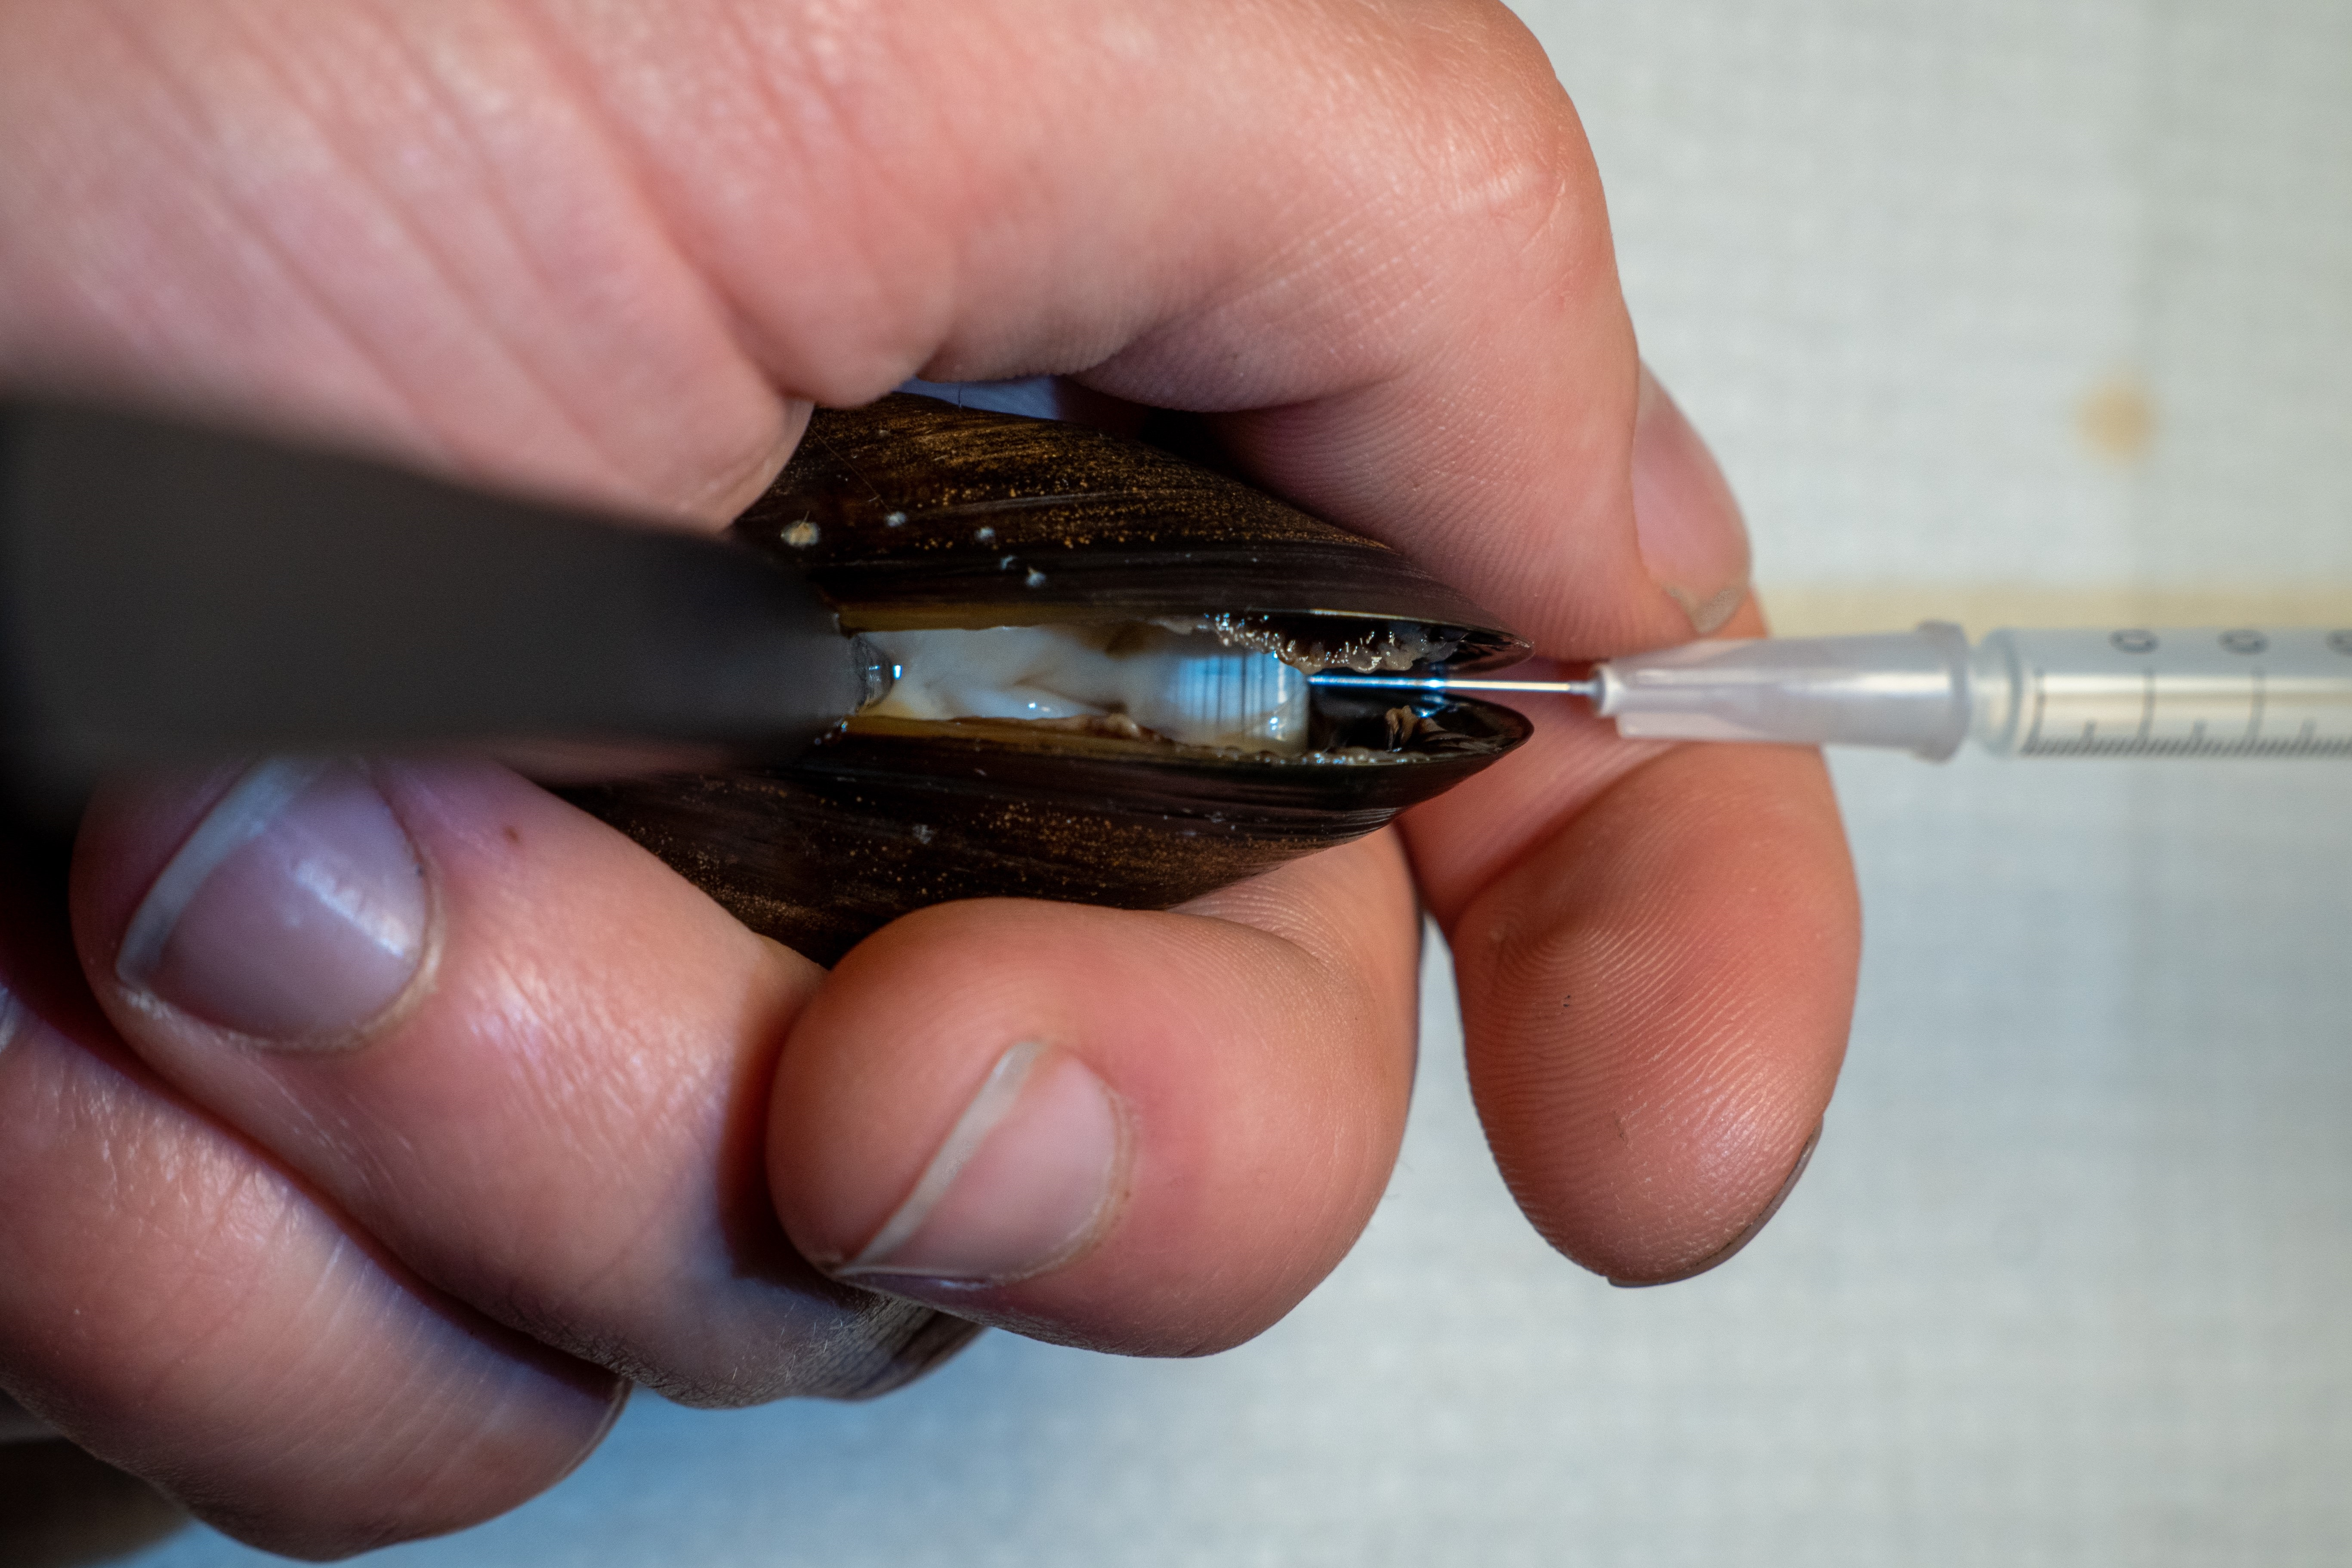
\includegraphics[width=\textwidth]{figures/Sampling technique/hands colors centered.jpg}
        \caption{The mussel grip and needle alignment employed, seen from the operators perspective. }
        \label{sfig:c}
    \end{subfigure}
    \hfill
    \begin{subfigure}[b]{.45\textwidth}
        \centering
        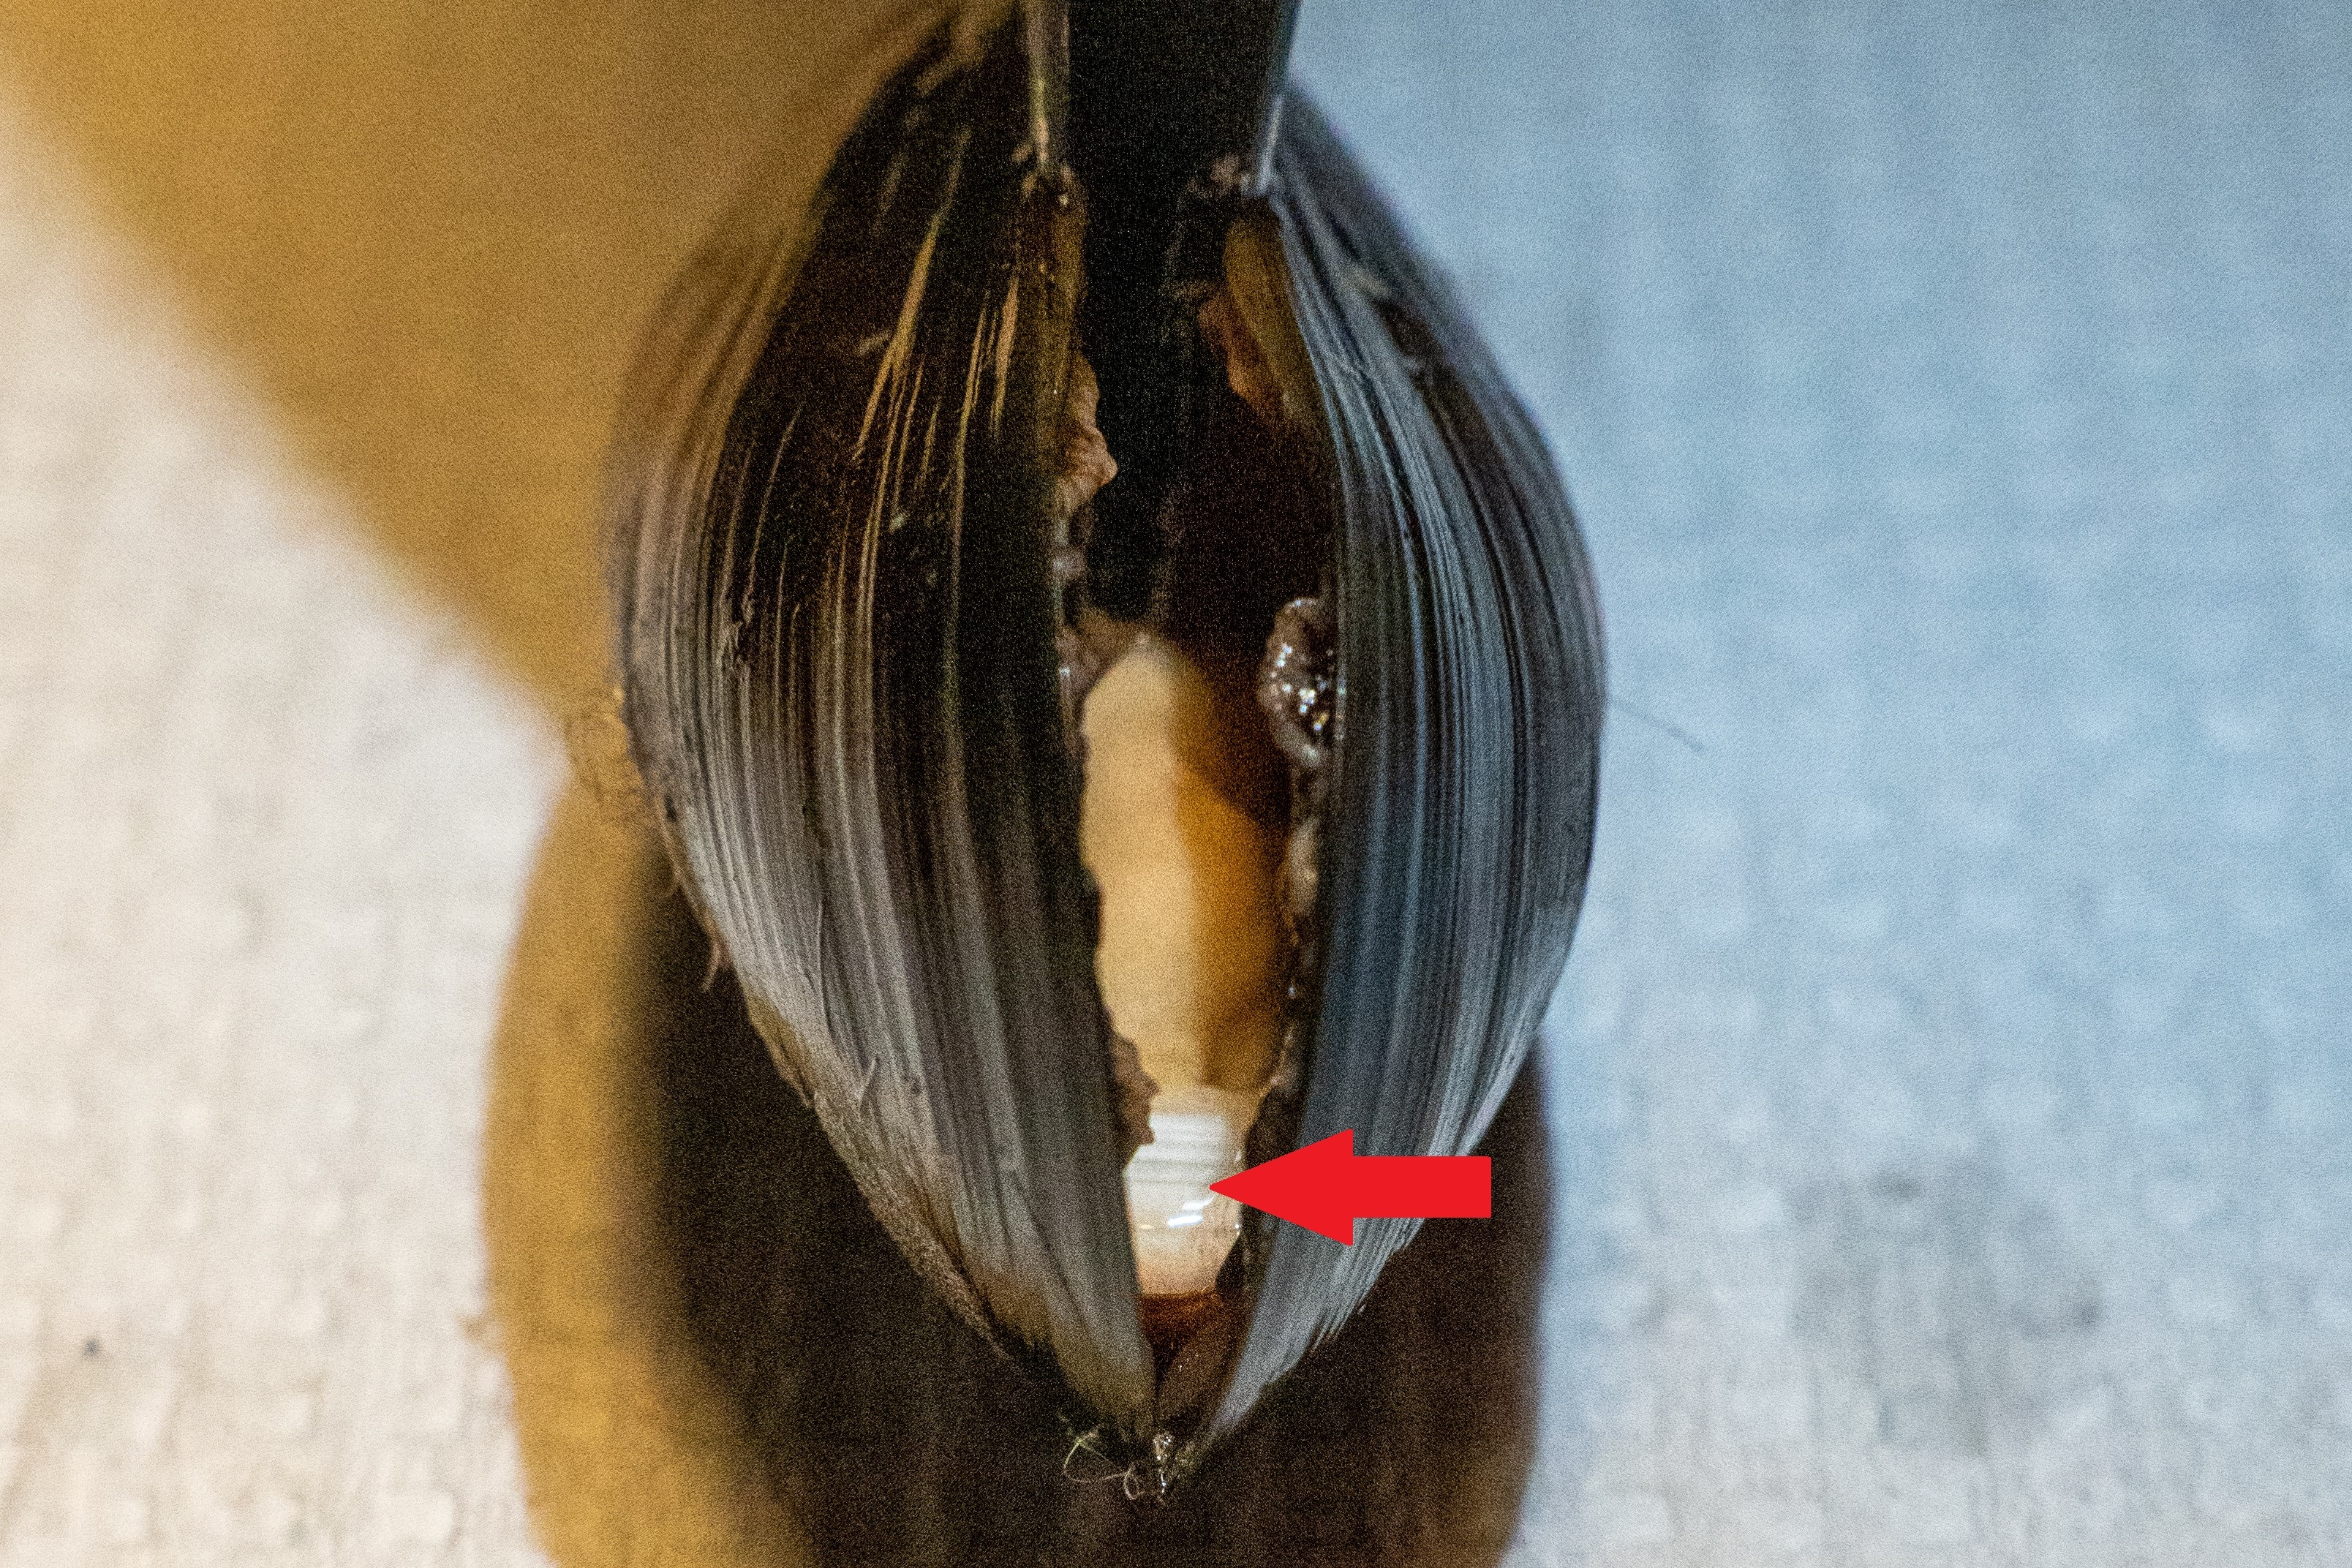
\includegraphics[width=\textwidth]{figures/Sampling technique/possible match.jpg}
        \caption{Mussel with visible posterior adductor muscle (red arrow) where the mantel was cut.}
        \label{sfig:d}
    \end{subfigure}
    \caption{An illustration of the method employed to extract hemolymph from M. edulis in order to avoid off-target withdrawal of fluid from surrounding tissues or enclosed seawater.}
    \label{fig:Hemolymph_sampling_illustration}
\end{figure}


What mean purity of hemocytes was obtained from the hemolymph sampling technique employed? Use the \% of plot in hemocyte gate from all samples run on flow cytometer before or during (or both) sampling period.

Adobe\textsuperscript{\textregistered} Lightroom Classic 12.0 
Sony ILCE A6400 with E-mount, lense:  
\chapter{Results}
\label{chap:results_method_development}

\section{Haemocyte medium}
The following section presents results from two experiments that were conducted to explore the suitability of three haemocyte media for applications in flow cytometric assays. They are compared with regard to their ability to inhibit haemocyte aggregation, without affecting the viability of haemocytes.

\subsection{Inhibition of haemocyte aggregation}
The proportions of aggregated haemocytes in \acrshort{mpss}, \acrshort{acb} and \acrshort{mas} are plotted against time post-withdrawal in Figure \ref{fig:aggregation}, together with their predicted mean proportions, or more accurately: the predicted proportion of aggregated haemocytes in mussels with random effects $\gamma_{0i}$ and $\gamma_{1i}$ = 0. Predictions were made from the estimated fixed effects in order to address the marginal effect of "Buffer" on the population-averaged proportions. The estimated regression coefficients of the generalized linear mixed effect model is presented in Table \ref{tb:regression_table}, while the fixed effect sub-models are shown in (\ref{eq:mixed_submodels}).

\begin{equation}
    \label{eq:mixed_submodels}
    y_{ij} = \begin{cases}
        \dfrac{1}{1 + e^{-(-1.7192 + 0.5516 \times log(t_{ij}))}},  & i \: \text{in MPSS group}, \\
        \dfrac{1}{1 + e^{-(-6.9842 + 1.8400 \times log(t_{ij}))}},  & i \: \text{in ACB group}, \\
        \dfrac{1}{1 + e^{-(-7.7198 + 2.0138 \times log(t_{ij}))}},  & i \: \text{in MAS group} \\
    \end{cases}
\end{equation}

Figure \ref{fig:aggregation}D unambiguously demonstrates that both \acrshort{acb} and \acrshort{mas} exerted an immediate decelerating effect on the rate of haemocyte aggregation. This inhibitory effect is evident from the estimated differences in slopes and intercepts from the MPSS sub-model, which were significantly different from zero (see Table \ref{tb:regression_table}). Since the effect sizes are a bit challenging to interpret from the isolated coefficients, the linear predictors of the three sub-models are evaluated on link scale in Figure \ref{fig:LogOdds}, i.e. as predictors for the log odds of the proportion of aggregated haemocytes ($log P(y_{ij} = 1) / P(y_{ij} = 0)$).

\begin{figure}[!ht]
    \centering
    \includegraphics[width=1.0\textwidth]{figures/Method development/Propagg x4 plot.pdf}
    \caption{\textbf{Inhibition of hemocyte aggregation from withdrawing samples into three different anticoagulant buffers.} The proportion of aggregated hemocytes is plotted against time from haemolymph withdrawal after diluting samples in an equal volume of \textbf{A)} Marine Physiological Saline Solution (\acrshort{mpss}, n=8), \textbf{B)} Modified Alsever's Solution (\acrshort{mas}, n=8) or \textbf{C)} Anticoagulant Buffer (\acrshort{acb}, n=8).  \textbf{D)} The same data is combined into one scatter-plot with regression curves representing the mean proportions of aggregated haemocytes in \acrshort{mpss} (\protect\darkgraycircle), \acrshort{mas} (\protect\lysegraacircle) and \acrshort{acb} (\protect\graycircle), as predicted from the fitted mixed logistic regression model. Note that data-points have been jittered on the x-axis to prevent overlap.}
    \label{fig:aggregation}
\end{figure}

\begin{table}[H]
	\centering
	\caption{Parameter estimates of the fitted mixed logistic regression model and their 95\% confidence intervals. Marginal and conditional R$^{2}$-values are presented as parameters of model fit, together with the model's residual deviance.}
	\label{tb:regression_table}
	\begin{tabular}{llllc}
        \toprule
	\textbf{Covariate} & \textbf{Symbol} & \textbf{Estimate$^{b}$} & \textbf{95\% CI$^{a}$} & \textbf{S.E.}\\
		\midrule
  \emph{Intercept}                          & $\alpha_1$ & -1.72*     & [-3.24, -0.202] & 0.740 \\
  \emph{log(t)}                             & $\beta_1$  & 0.552**    & [0.189, 0.915]  & 0.177 \\
  \emph{Buffer$_{ACB}$}                     & $\alpha_2$ & -5.27***   & [-7.41, -3.11]  & 1.05  \\
  \emph{Buffer$_{MAS}$}                     & $\alpha_3$ & -6.00***   & [-8.18, -3.86]  & 1.06  \\
  \emph{log(t)} $\cdot$ \emph{Buffer$_{ACB}$} & $\beta_2$& 1.29***    & [0.775, 1.80]   & 0.251 \\
  \emph{log(t)} $\cdot$ \emph{Buffer$_{MAS}$} & $\beta_3$& 1.46***    & [0.950, 1.98]   & 0.253 \\
  \emph{SD}$(\gamma_{0i})$                  & $\tau_0^2$ & 2.09       & [1.57, 2.91]    & -     \\
  \emph{SD}$(\gamma_{1i})$                  & $\tau_1^2$ & 0.500      & [0.379, 0.694]  & -     \\
  &&& \\
  \multicolumn{5}{l}{Marginal R$^{2}$ = 0.87$^{c}$} \\
  \multicolumn{5}{l}{Conditional R$^{2}$ = 0.98$^{c}$} \\
  \multicolumn{5}{l}{Residual deviance: 13498 on 98 degrees of freedom} \\
		\bottomrule
  \multicolumn{5}{l}{\footnotesize $^{a}$Computed 95\% confidence intervals based on Likelihood Ratio Test of the profile likelihood.} \\
  \multicolumn{5}{l}{\footnotesize $^{b}$ *, **, *** indicates statistical significance on 95\%, 99\% and 99.9\% confidence levels, respectively.} \\
  \multicolumn{5}{l}{\footnotesize Confidence levels were obtained from z-statistics of the asymptotic Wald test.} \\
    \multicolumn{5}{l}{\footnotesize $^{c}$Calculated according to the method proposed by Nakagawa and Schielzeth (2013).} \\
	\end{tabular}
\end{table}

\begin{figure}[!ht]
    \centering
    \includegraphics[width=1.0\textwidth]{figures/Method development/Log Odds plot.pdf}
    \caption{The log odds of the proportion of aggregated haemocytes plotted against time (min) after haemolymph withdrawal, when haemolymph samples were withdrawn into Marine Physiological Saline Solution (MPSS), Anticoagulant Buffer (ACB) or Modified Alsever's Solution (MAS). The three curves illustrates the logit-scale predictors of the fitted mixed logistic regression model for the three buffers.}
    \label{fig:LogOdds}
\end{figure}

Given the that the predicted proportion of aggregated haemocytes is 0.50 when the log odds is equal to zero, Figure \ref{fig:LogOdds} shows that 1/2 of the haemocytes withdrawn into \acrshort{mpss} had aggregated within 23 minutes post-withdrawal. This interpretation is valid for mussels where the random effects of time; $\gamma_{0i}$ and $\gamma_{1i}$ = 0. For samples withdrawn into \acrshort{acb} or \acrshort{mas} on the other hand, the cells did not achieve this degree of aggregation until 45 and 46 minutes post-withdrawal, respectively. The three log odds curves depicted in Figure \ref{fig:LogOdds} shows that the inhibitory effects of \acrshort{acb} and \acrshort{mas} were modelled through their significantly lower y-intercepts compared to the \acrshort{mpss} sub-model (Table \ref{tb:regression_table}). Since these estimates were significant after accounting for within-mussel correlations (<.001), we can conclude that \acrshort{edta} is an effective haemocyte anticoagulant on the short term.

The effect was largest during the initial 15-20 minutes, before the degree of aggregation slowly approached that of \acrshort{mpss} around 60 minutes post-withdrawal. In haemolymph samples withdrawn into \acrshort{acb} or \acrshort{mas}, the mean proportions of aggregated haemocytes after 15 minutes were 0.14 95\% CI [0.07, 0.22] and  0.20 95\% CI [0.07, 0.32], respectively. There were no significant differences between the buffers with \acrshort{edta}, but both \acrshort{acb} and \acrshort{mas} had significantly lower proportions at this timepoint compared to samples withdrawn into cold \acrshort{mpss} (0.48 95\% CI [0.39, 0.56]).

\subsection{EDTA cytotoxicity}
 The mean percentages of necrotic hemocytes in \acrshort{mpss}, \acrshort{acb} and \acrshort{mas} after 15 minutes, 2 hours and 20 hours incubation are presented in Figure \ref{fig:BufferViability}, with error bars representing 95\% confidence intervals around group means. Within group differences in means at the three incubation periods are presented Table \ref{tb:Paired_ttests}.

\begin{figure}[H]
    \centering
    \includegraphics[width=0.75\textwidth]{figures/Method development/EDTA cytotoxicity.pdf}
    \caption{The mean percentages of TO-PRO$^{TM}$-3 Iodide positive hemocytes after 15 minute, 2 hours and 20 hours incubation in Marine Physiological Saline Solution (\, \protect\lysegraabox, \ n=8), Anticoagulant Buffer (\, \protect\customgraybox, \ n=8) and Modified Alsever's Solution (\, \protect\darkgraybox, \ n=8). Error bars represent 95\% confidence intervals around group means, *, **, *** above error bars denotes confidence level of one-tailed two sample t-test comparisons with the \acrshort{mpss} control group, while asterisks above horizontal lines represent \acrshort{acb} vs. \acrshort{mas} comparisons. NS: Not Significant.}
    \label{fig:BufferViability}
\end{figure}

The difference between the negative control group (\acrshort{mpss}) and the two \acrshort{edta}-containing buffers were not significantly different from zero after 15 minute incubation. But as the incubation period was increased to 2 and 20 hours, the percentages of necrotic haemocytes in \acrshort{acb} and \acrshort{mas} increased relative to the negative control group. After 2 hours incubation, there were 0.40\% and 0.27\% more necrotic haemocytes in \acrshort{acb} (t(14) = 4.29, p<.001) and \acrshort{mas} (t(14) = 2.86, p=.006) compared to cold \acrshort{mpss}, respectively. After 20 hours incubation, these differences had increased to 6.96\% (t(14) = 3.78, p=.003) and 5.12\% (t(14) = 4.82, p<.001).

The mean percentage of necrotic haemocytes increased significantly with the incubation period in both MAS and ACB (Table \ref{tb:Paired_ttests}). Since the concentration of EDTA was constant across all timepoints, this increase was dose-dependent as the exposure duration was the only variable factor. There were no significant increase in the percentage of necrotic haemocytes in MPSS from 15 minutes to 2 hours incubation, but a significant increase of 1.184\% was observed after 20 hours (p<.026).

\begin{table}[h!]
\centering
	\caption{Paired two-tailed t-tests were used to assess wether the percentages of necrotic haemocytes increased with incubation time within each group. The difference between means at t = 15 min, 2 hours and 20 hours are presented with 95\% confidence intervals and the belonging p-value.}
	\label{tb:Paired_ttests}
        \resizebox{\linewidth}{!}{
	\begin{tabular}{c|ccccc}
		\toprule
		\multirow{2}{*}{Buffer} & \multicolumn{2}{c}{\textbf{Paired t-test comparison}} & \multirow{2}{*}{Difference (\%)} & \multirow{2}{*}{95\% CI} & \multirow{2}{*}{Pr(T > $\mid$ t $\mid)$} \\
		& Incubation \emph{t} & Incubation \emph{t - 1} & & & \\
		\midrule
     \multirow{2}{*}{MPSS} &  2 hours  &  15 min  & -0.018 & [-0.023, -0.015] & .78 \\
     &  20 hours &  2 hours & 1.184  & [1.157, 1.211]   & .026 \\
    \multirow{2}{*}{ACB} &   2 hours  &  15 min  & 0.438  & [0.433, 0.444]   & .00187 \\
       &   20 hours &  2 hours & 7.742  & [7.627, 7.857]   & .00324 \\
    \multirow{2}{*}{MAS} &   2 hours  &  15 min  & 0.319  & [0.313, 0.324]   & .00690 \\
        &   20 hours &  2 hours & 6.037  & [5.970, 6.105]   & <.001 \\
		\bottomrule
	\end{tabular}
 }
\end{table}


\subsection{Cytotoxicity of acidic haemocyte medium pH}
The mean percentage of early and late apoptotic haemocytes after 15 minutes incubation in non-adjusted Modified Alsever's Solution (\acrshort{namas}, pH = 6.1) and Anticoagulant Buffer (ACB, pH = 7.6) is presented as bargraphs in Figure \ref{fig:pH_Apo}, with error bars representing 95\% confidence intervals around group means. 

\begin{figure}[H]
    \centering
    \includegraphics[width=0.5\textwidth]{figures/Method development/Apo15 pH.pdf}
    \caption{The mean percentage of early apoptotic (Apo15$^{+}$/ToPro3$^{-}$) and late apoptotic haemocytes (Apo15$^{+}$/ToPro3$^{+}$) after 15 minutes incubation in Anticoagulant Buffer (\, \protect\customgraybox, \ n=18) and non-adjusted Modified Alsever's Solution (\, \protect\darkgraybox, \ n=18). Error bars represent 95\% confidence intervals around group means. Asterisks *, **, *** denotes confidence level of one-tailed two sample t-test comparisons.}
    \label{fig:pH_Apo}
\end{figure}

Haemocytes that were incubated in the acidic MAS buffer showed a significant induction of apoptosis relative to samples kept in ACB. The mean percentage of early apoptotic haemocytes in naMAS were 53 times higher than in ACB (t(17) = 6.04, p<.001), while that of late apoptotic haemocytes were 31 times higher (t(17) = 3.57, p=.00117). The percentages of early and late apoptotic haemocytes in ACB were consistently low, with mean percentages of 0.165$\pm{0.2}$\% and 0.144$\pm{0.09}$\%, respectively.

\section{Development of a flow cytometric differential count}
This section presents the results of several experiments that were conducted in order to develop and validate a flow cytometric differential count of the cell types present in the haemolymph of \emph{M. edulis}. Section \ref{subsection:CytCar} presents a cytological characterization of the haemocytes according to i.a., cell size, granularity and staining affinities in accordance with the current scientific practice in invertebrate immunology. The flow cytometric characterization in section \ref{subsection:Results_FlowChar} presents the subpopulations of haemocytes that were separated according to FSC (relative size) and side scatter (internal complexity), and set these results in context of the cytologically defined cell types. The next section (\ref{subsection:evidence}) presents results from two experiments that were aimed to uncover the relationship between the cytologically defined cell types and the subpopulations discernible by light scatter measurements. Lastly, the gating strategy for the differential count is presented with proof of concept. The results are presented and discussed consecutively since each subsequent section builds on the preceding.

\subsection{Cytologic characterization of \emph{M. edulis} hemocyte subpopulations}
\label{subsection:Results_cytchar}
The hemolymph of \emph{Mytilus edulis} comprised a mixed population of cells differing in size, granularity, morphometrics and Wright's-Giemsa staining profiles. If the haemocytes were allowed to spread prior to fixation and staining, the diversity further expanded as cells took on a variety of shapes and/or developed cytoplasmic extensions. From these morphological criteria, a total of three distinct cell types could be identified by light microscopy.

Based on the basophilic or eosinophilic nature of their granules and other cytoplasmic contents, cytologic staining with 3 \% Wright's-Giemsa or the Hemacolor\textsuperscript{\textregistered} kit gave rise to two distinct staining profiles: basophilic and eosinophilic haemocytes. The cytoplasm of eosinophilic hemocytes (Figure \ref{fig:celltypes}, K-O) were densely packed with pink to dark purple granules of varying size and abundance. Hence, they are referred to as eosinophilic granulocytes herein. Their individual granules were usually not distinguishable in a non-spread state, but instead gave their cytoplasm an irregular pink color (Figure \ref{fig:celltypes}, K and O). These haemocytes had cell diameters in the range of 6-16 \micro m, with a mean of 9.06$\pm1.25$ \micro m. Two strikingly homogeneous features of this cell type was a small acentrically located nucleus, and a regular spherical outline in a non-spread state. With abundant pink cytoplasm making up the majority of the cells' surface area - even in the smallest specimens - the eosinophilic granulocytes could also be characterized by a low nuclear-cytoplasmic ratio (N:C ratio). If not fixed and stained before smearing - or within minutes of applying haemolymph to a glass slide - eosinophilic granulocytes were almost exclusively observed as spread cells. 

\begin{figure}[H]
    \centering
    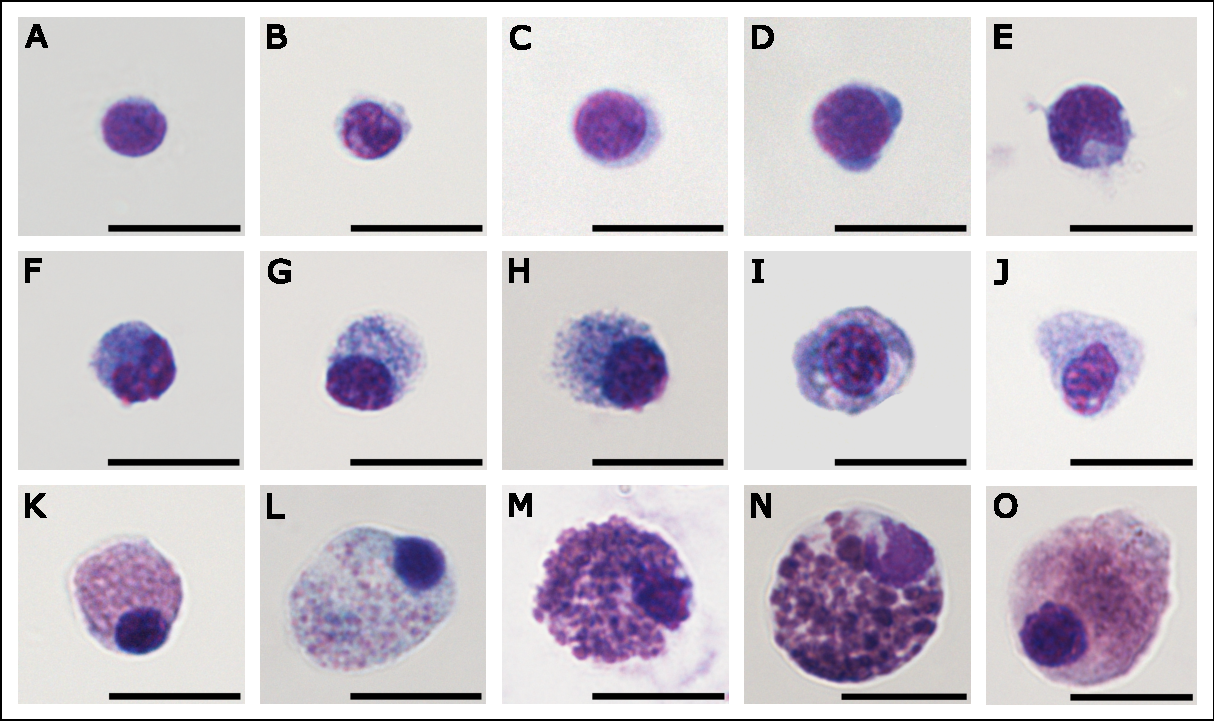
\includegraphics[width=1.0\textwidth]{figures/Anatomy/cell types brightfield updated 2.pdf}
    \caption{100$\times$ brightfield micrographs of the three haemocyte types found in the haemolymph of \emph{Mytilus edulis}, fixed and stained on glass slides with the Hemacolor\textsuperscript{\textregistered} kit before the hemocytes had time to spread notably. \textbf{(A-E)} Blast-like hyaline basophils. \textbf{(F-J)} Basophilic granulocytes. \textbf{(K-O)} Eosinophilic granulocytes. Samples were withdrawn into \acrshort{mpss} (1:1), scale bars = 10 \micro m.}
    \label{fig:celltypes}
\end{figure}

Compared to the eosinophilic granulocytes, the basophilic hemocytes encompassed a more heterogeneous population. Common to all of them were a larger nucleus that occupied more of the cells' total surface area (higher N:C ratio). The shape of which varied from spherical to oval, or had a distinct bean-shaped or irregular outline. But judged from the morphological criteria of cell size, granularity and N:C ratio, there were essentially two distinct subpopulations of basophilic haemocytes: one population of small hyaline blast-like haemocytes (5.63 $\pm{0.72}$ \micro m) displaying only a marginal rim of dove blue cytoplasm and no apparent cytoplasmic granules (Figure \ref{fig:celltypes}, A-E), and one population of larger haemocytes (8.07 $\pm{1.25}$ \micro m), displaying abundant basophilic cytoplasm with varying degrees of cytoplasmic granulation and vacuolation (Figure \ref{fig:celltypes}, F-J). The basophillic granules appeared much smaller than those of the eosinophilic granulocytes, and were usually not very conspicuous unless haemocytes were subjected to osmotic swelling prior to fixation and staining. Under differential interference contrast (DIC) illumination however, their granules created highly irregular surface topographies in spread cells that could be observed without such treatment. On the basis of these morphological differences, the basophilic haemocytes were subdivided into blast-like haemocytes and basophilic granulocytes herein. 

\begin{figure}[H]
    \centering
    \includegraphics[width=1.0\textwidth]{figures/Anatomy/diameters scaled density plot.pdf}
    \caption{Size distribution of \protect\dimgraybox \ small blast-like basophils (n=154), \protect\lightgraybox \ basophilic granulocytes (n=821), \protect\lysegraabox \ eosinophilic granulocytes (n=1030) and \protect\whitebox \ the total haemocyte population of \emph{Mytilus edulis} (n=2005). The diameters of 100 formaldehyde-fixed haemocytes were measured in each of 20 individual mussels, and the density was scaled to the number of observations of each cell type.}
    \label{fig:Diameters}
\end{figure}

The size distributions of the three haemocyte types are shown as three kernel-smoothened density plots in Figure \ref{fig:Diameters}, together with that of the total haemocyte population. The densities have been scaled to the number of observations of each cell type, such that their relative proportions can be visualized. In the 20 adult mussels examined here, the small blast-like basophils were the least abundant cell type, making up 7.9 $\pm{5.6}$\% of the total haemocyte population. In 14 out of 20 mussels, the blast-like basophils were followed by the basophilic granulocytes, with a mean relative proportion of 40.7 $\pm{12.9}$\%. In spite of constituting similar proportions as the basophilic granulocytes in several mussels, the eosinophilic granulocytes were the most abundant cell type in the haemolymph of \emph{M. edulis}, constituting 51.5 $\pm{15.3}$\% of the total haemocyte population, on average. The relative proportions of basophilic and eosinophilic granulocytes did however vary to a large extent between individual mussels, as reflected by their standard deviations.

\subsection{Flow cytometric characterization of haemocyte subpopulations by light-scatter}
\label{subsection:Results_FlowChar}
A maximum of three distinct subpopulations could be separated according to Forwards scatter (FCS) vs. Side scatter (\acrshort{ssc}) in suspensions of living haemocytes. These comprised one subpopulation of events with low \acrshort{fsc}- and \acrshort{ssc}-values, one with high \acrshort{fsc}- and intermediate \acrshort{ssc}-values and one with high \acrshort{fsc} and \acrshort{ssc}. The aforementioned subpopulations correspond to clusters 1, 2 and 3 in Figure \ref{fig:fsc_vs_ssc}, where the haemocytes of three representative mussels have been displayed with \acrshort{ssc} on logarithmic and linear scales.

The adjunct histograms in Figure \ref{fig:fsc_vs_ssc}A and B clearly illustrates that the three clusters of events are separated according to log \acrshort{ssc}, while there is substantial overlap between cluster 2 and 3 with regard to \acrshort{fsc}. The latter feature was consistent across all mussels, while the degree of separation according to log \acrshort{ssc} was subject to individual variation. In this regard, the haemolymph sample presented in \ref{fig:fsc_vs_ssc}B represents a typical mussel, i.e., with cluster 2 and 3 incompletely separated according to log \acrshort{ssc}. The samples presented in \ref{fig:fsc_vs_ssc}A and C represents the extreme ends of this variation, with complete separation and complete overlap, respectively.

Since \acrshort{fsc} and \acrshort{ssc} can be interpreted as relative measures of cell size and internal complexity, these results suggests that the haemolymph of \emph{M. edulis} are comprised of three cell types that are distinguishable according to size and internal complexity. The events populating cluster 1 exhibited low \acrshort{fsc}- and \acrshort{ssc}-values relative to cluster 2 and 3, indicating that it is populated by haemocytes that are both smaller and less complex than the rest of the haemocytes. If \acrshort{ssc} is interpreted more specifically in terms of haemocyte characteristics, the events populating cluster 2 and 3 most likely correspond to large semi-granular haemocytes and large granulocytes, respectively.

\begin{figure}[ht!]
    \centering
    \includegraphics[width=1.0\textwidth]{figures/Gating strategy/30k scatter profiles musc.pdf}
    \caption{\textbf{Haemocyte subpopulations distinguishable according to \acrshort{fsc} and \acrshort{ssc} measurements with the BD Accuri C6 Plus Benchtop Flow Cytometer.} The light-scatter profiles of three representative adult mussels are displayed with \acrshort{ssc} on logarithmic \textbf{(A-C)} and linear \textbf{(D-F)} scales to illustrate the observed variation in the degree of separation between cluster 2 and 3. Adjunct histograms were included to underline the degree of separation from the individual parameters.}
    \label{fig:fsc_vs_ssc}
\end{figure}

\subsection{Relating cytologically defined cell types to light-scatter profiles}
\label{subsection:evidence}
\subsubsection{Flow cytometric characterization of haemocytes pre-separated by isopycnic centrifugation }
Formaldehyde-fixed haemocytes separated into three distinct cell-bands on the 15/33\%, 38/43\% and 43/90\% gradient interfaces of the discontinuous Percoll gradients. As shown in Figure \ref{fig:Percoll-tubes}, the two upmost bands exhibited a similar blue coloration, while the band located on the 43/90\% interface had a darker purple color. The latter consisted of 96.9$\pm{0.9}$\% eosinophilic granulocytes, with a few basophillic granulocytes scattered among them. From the cell bands located at the 15/33\% interface, a populations of 96.3$\pm{0.2}$\% basophillic haemocytes were isolated. The majority of these cells were basophilic granulocytes (87.5$\pm{1.2}$\%), with a smaller fraction of blast-like basophils (8.8$\pm{1.5}$\%). The middle bands did not yield any of the cell types in high purity, but were predominantly populated by basophilic granulocytes (72.7$\pm{1.5}$\%) with numerous small dark granules.

\begin{figure}[H]
    \centering
    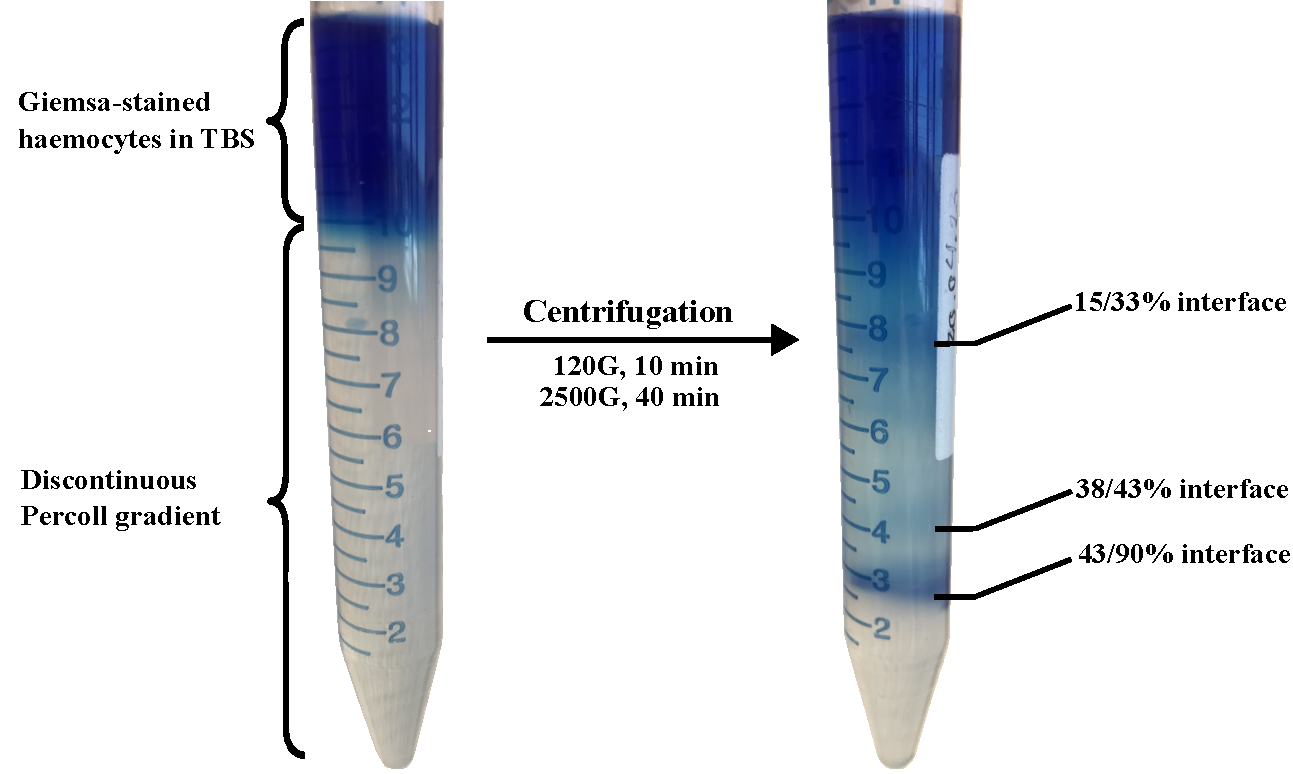
\includegraphics[width=.75\textwidth]{figures/Method development/Percoll tubes.pdf}
    \caption{\textbf{Formaldehyde-fixed haemocytes pre-stained with Giemsa were separated by isopycnic centrifugation on discontinuous Percoll gradients.} Haemocytes settled into three distinct cell bands on the 15/33\%, 38/43\% and 43/90\% gradient interfaces.}
    \label{fig:Percoll-tubes}
\end{figure}

The light scatter profiles of the three isolated cell fractions are depicted in Figure \ref{fig:Percoll-dotplots}, together with that of the unseparated haemocytes. As shown in Figure \ref{fig:Percoll-dotplots}A, the pooled haemocyte were not readily distinguishable as three separate subpopulations prior to centrifugation. Since the relative size and complexity of the three cell types vary slightly between individual mussel, this is a common phenomenon when haemolymph from two or more mussels are pooled together. A more distinct clustering was however seen among haemocytes isolated from the middle cell-band (\ref{fig:Percoll-dotplots}C), where the relative proportions of eosinophilic granulocytes (18.4\%) and blast-like basophils (7.8\%) were lower.

\begin{figure}[H]
    \centering
    \includegraphics[width=1.0\textwidth]{figures/Method development/PERCOLL SEP II.pdf}
    \caption{\textbf{Flow cytometric analysis of the isolated cells types of \emph{M. edulis} haemolymph after separation by isopycnic centrifugation.} Two pools of formaldehyde-fixed haemocytes were separated by density-dependent centrifugation after the method of Friebel and Renwrantz (1994), and the isolated fractions were analyzed by flow cytometry and light microscopy. FSC vs. log SSC density plots depicts one of the pools prior to centrifugation \textbf{(A)} and after separating into three distinct cell-bands on the gradient interfaces \textbf{(B-D)}. The enriched fractions (> 96\%) of eosinophilic granulocytes \textbf{(B)} and basophilic haemocytes \textbf{(D)} are overlayed in \textbf{(E)}, with micrographs of the respective layers presented in \textbf{(F)}. F-1: eosinophilic granulocytes; F-2: basophilic granulocytes; scale bars = 10 \micro m. }
    \label{fig:Percoll-dotplots}
\end{figure}

The eosinophilic granulocytes formed a dense cluster of events exhibiting high FSC- and SSC-values (Figure \ref{fig:Percoll-dotplots}B). This is consistent with the expected light scatter profile of this cell type, since they represent highly granulated cells with large cell diameters. The two basophilic cell types from the upper cell band were unambiguously separated from the eosinophilic granulocytes according to SSC, where only a small number of cells exceeded values > 1$\times 10^{6}$ (Figure \ref{fig:Percoll-dotplots}D). This relationship is clearly demonstrated by the overlayed dotplot in Figure \ref{fig:Percoll-dotplots}E, where the eosinophilic granulocytes are shown in pink.

\subsubsection{Identification of eosinophilic granulocytes by eosin fluorescence}
Formaldehyde-fixed haemocytes stained with 0.5\% eosin were separated into distinct eosin$^{bright}$ and eosin$^{dim}$ populations by flow cytometric measurements of eosin fluorescence (Figure \ref{fig:eosin_exp2}B and C). The degree of separation varied to a large extent between individual mussels, but the \acrshort{mfi} of eosin$^{bright}$ events were 11$\pm{9}$ times higher than that of eosin$^{dim}$ events on average. The difference in fluorescent intensity between eosinophilic and basophilic granulocytes is illustrated in Figure \ref{fig:Eosin_fluorescence_B2A}, where Giemsa-stained haemocytes have been imaged by epifluorescence microscopy with a B-2A filtercube (Em: $\geq$ 515 nm; exposure: 250 msec; gain: 3.4).

\begin{figure}[H]
    \centering
    \begin{subfigure}[b]{.45\textwidth}
        \centering
        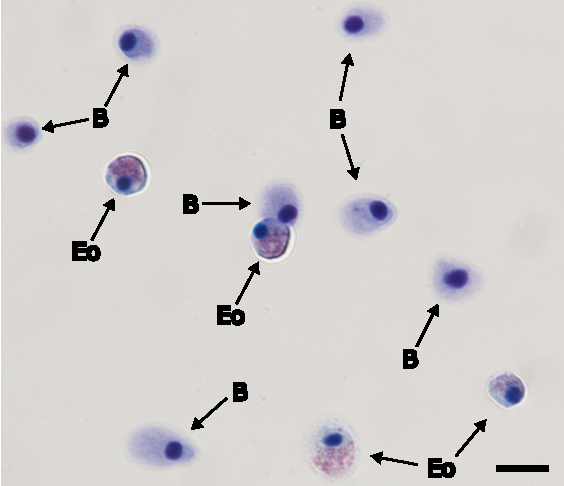
\includegraphics[width=\textwidth]{figures/Method development/B2A eosin fluorescence/Epi eosin fluorescence.pdf}
        \caption{Hemocytes imaged under brightfield illumination.}
        \label{ffig:a}
    \end{subfigure}
    \hfill
    \begin{subfigure}[b]{.45\textwidth}
        \centering
        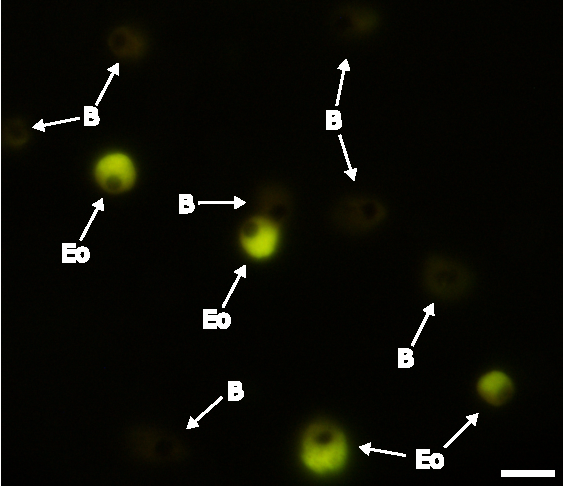
\includegraphics[width=\textwidth]{figures/Method development/B2A eosin fluorescence/Brightfield eosin fluorescence.pdf}
        \caption{Haemocytes imaged by epifluorescence microscopy with a B-2A filtercube.}
        \label{ffig:b}
    \end{subfigure}
    \caption{\textbf{Eosinophilic granulocytes are distinguished from the two basophilic cell types according to eosin fluorescence ($\geq$ 515 nm).} Formaldehyde-fixed haemocytes stained in 0.5\% eosin and 3\% Giemsa were imaged at $\times$60 magnification under \textbf{a)} brightfield illumination and \textbf{b)} by epifluorescence microscopy with a B-2A filter cube. The slide was mounted with Eukitt\textsuperscript{\textregistered} and coverslipped prior to microscopy. Eo: eosinophilic granulocyte; B: basophilic haemocyte; scale bars = 10 \micro m. }
    \label{fig:Eosin_fluorescence_B2A}
\end{figure}

The pooled sample depicted in Figure \ref{fig:eosin_exp2}A were unambiguously separated into three distinct haemocyte subpopulations according to FSC and SSC. These subpopulations are equivalent to cluster 1-3 in samples of living haemocytes (see Figure \ref{fig:fsc_vs_ssc}). When the eosin$^{bright}$ events were back-gated to bivariate plots of FSC vs. SSC, they invariably corresponded to the subpopulation with high FSC- and SSC-values, i.e., cluster 3. (see Figure \ref{fig:eosin_exp2}D). This is clearly demonstrated by comparing Figure \ref{fig:eosin_exp2}A and D, where the eosin$^{bright}$ events are shown in pink.

The correlation between eosin$^{bright}$ events (\%) and the percentage of eosinophilic granulocytes were analyzed by simple linear regression on order to verify the linearity of response. The analysis showed that eosin$^{bright}$ events (\%) recorded by flow cytometry significantly predicted the percentage of eosinophilic granulocytes($\beta$ = 1.06656, 95\% CI [0.96, 1.17], t(8) = 23.3, p<.001), with a mean absolute error of 1.71$\pm{1.6}$\%. The data is presented in Figure \ref{fig:eosin_exp2}E, together with the fitted linear regression model (R$^{2}$ = 0.99, F(1, 8) = 541, p<.001).

\begin{figure}[H]
    \centering
    \includegraphics[width=1.0\textwidth]{figures/Method development/Eosin with method validation.pdf}
    \caption{\textbf{Identification eosinophilic granulocytes on FSC vs. SSC dotplots according to log eosin fluorescence (518-548 nm).} Ten formaldehyde-fixed haemolymph samples were stained with 0.5\% eosin and recorded on the flow cytometer right thereafter \textbf{(A)}. Haemocyte events were gated according to log eosin fluorescence vs. SSC-A \textbf{(B)} and the eosin$^{bright}$ events were gated univariately \textbf{(C)}. The eosin$^{bright}$ events were back-gated to show their light scatter profile relative to eosin$^{dim}$ events \textbf{(D)}. The simple regression of eosin$^{bright}$ events (\%) vs. eosinophilic granulocytes (\%) determined from 1000-cell differential counts are shown in \textbf{(E)}, regression line: y$_{i}$ = -3.20042 + 1.06656x$_{i}$.}
    \label{fig:eosin_exp2}
\end{figure}

\subsection{Flow cytometric differential haemocyte count}


\begin{figure}[H]
    \centering
    \includegraphics[width=1.0\textwidth]{figures/Gating strategy/GatestratGY SSC Calcein PNG.pdf}
    \caption{ \textbf{Differential haemocyte count gating strategy}.}
    \label{fig:DHC_gatestrat}
\end{figure}





\begin{figure}[H]
    \centering
    \includegraphics[width=1.0\textwidth]{figures/Gating strategy/SSC Calcein validation.pdf}
    \caption{Correlation between the percentages of eosinophilic granulocytes \textbf{(A)}, basophilic granulocytes \textbf{(B)} and small blast-like basophils \textbf{(C)} from differential haemocyte counts performed by microscopy and flow cytometry (n=20). The three cell types were were differentiated according log SSC-A vs. log Calcein fluorescence (518-538 nm), as shown in the gating strategy in Figure 3.12. }
    \label{fig:DHC_lin}
\end{figure}

%  A: f(x) = -0.22708 + 0.98789x, 95\% CI [0.89148, 1.0842], MAE = 0.5755
% BG: f(x) = -3.13182 + 1.03003x, 95\% CI [0.96733, 1.0927], MEA = 2.263
% Eo: f(x) =  0.66011 + 1.02894x, 95\% CI [0.97425, 1.0836], MEA = 2.457


\newpage




\section{Scoring of necrotic haemocytes by flow cytometry}
\subsection{Determination of optimal TO-PRO-3 Iodide staining concentration}
Viable and \ce{MeOH}-killed haemocytes could be separated according to TO-PRO-3 Iodide fluorescence in the whole range of tested concentrations (30 nM - 8 \micro M). As shown in Figure \ref{fig:ToPro3_stain_opt}B, the resolution between ToPro3$^{-}$ and ToPro3$^{+}$ events increased with the TO-PRO$^{TM}$-3 Iodide concentration according to the log-logistic function shown in (\ref{eq:fitted.LL4}), with a marked stagnation > 1.2 \micro M. The model explained almost all the variation in the dataset (Pseudo-R$^{2}$ = 0.99, see table \ref{tb:loglogistic_ToPro3}), and should therefore be a good predictor of the expected resolution between necrotic and viable haemocytes in the tested range of TO-PRO$^{TM}$-3 Iodide.

\begin{equation}
\label{eq:fitted.LL4}
y_{i} = \dfrac{9890700}{1 + (x_i / 0.41655)^{-0.94088}} + \epsilon_i
\end{equation}

\begin{figure}[h]
    \centering
    \includegraphics[width=1.0\textwidth]{figures/Method development/ToPro3 LL4.pdf}
    \caption{\textbf{Experimental determination of the optimal TO-PRO$^{TM}$-3 Iodide concentration for a dye exclusion test of membrane integrity}. 10 aliquots of pooled methanol-killed (70\% \ce{MeOH}, 30 min) and viable haemocytes (1:1) were stained with different concentrations of TO-PRO$^{TM}$-3 Iodide (30 nM - 8 \micro M). 640 nm-exited fluorescence from \acrshort{dsdna}-bound TO-PRO$^{TM}$-3 Iodide were collected on the FL4 detector (675/25 nm) of the BD Accuri C6 Plus flow cytometer, recording 10.000 events from each sample after 15 and 30 minute incubation. \textbf{A)} ToPro3$^{-}$ and ToPro3$^{+}$ events were gated on log scale for each sample, \textbf{B)} and their difference in mean fluorescent intensity (MFI) after 15 (\protect\lysegraacircle) and 30 minutes (\protect\darkgraycircle) of incubation were plotted against the concentration of TO-PRO$^{TM}$-3 Iodide. Red line: fitted log-logistic regression model; blue dashed lines: prediction intervals.}
    \label{fig:ToPro3_stain_opt}
\end{figure}

The predicted difference in \acrshort{mfi} at 1.2 \micro M was 7.220.000 (arbitrary units), 95\% PI[6.170.000, 8.260.000]. Since the slope of function \ref{eq:fitted.LL4} decreased rapidly for x > 0.6, the predicted difference in MFI at x = 1.2 \micro M was contained within the prediction intervals for the rest of the function's range. Furthermore, the MFI of the ToPro3$^{-}$ populations increased abruptly at concentrations $\geq$ 2 \micro M (see Table \ref{tb:ToPro3_stainopt}), indicating a potential cytotoxic effect of either TO-PRO$^{TM}$-3 Iodide or the \acrshort{dmso} solvent at high concentrations.

Taken together, these results suggested that the potential gain from increasing the staining concentration above 1.2 \micro M was limited, and not completely free of risk. The resolution between viable and necrotic haemocytes was for all practical purposes sufficient in the range of 300 nm - 1.2 \micro M, but the resolution at 1.2 \micro M would simplify gating on a logarithmic scale. 1.2 \micro M TO-PRO$^{TM}$-3 Iodide was therefore preferred for scoring necrotic haemocytes by flow cytometry, together with 50 nM Calcein AM.

The results were also unambiguous regarding the incubation period. According to Figure \ref{fig:ToPro3_stain_opt}B, the resolution between viable and necrotic cells did not increase after the initial 15 minute incubation period. The MFI of necrotic haemocytes did increase somewhat in the extended incubation period, but the resolution remained unchanged due to a concurrent proportional increase among the viable haemocytes (see table \ref{tb:ToPro3_stainopt}, Appendix B). Extending the incubation period beyond 15 minutes would therefore be of little use.

\subsection{Gating strategy}
The finalized quadrant gating strategy for the Calcein AM/TO-PRO$^{TM}$-3 Iodide membrane integrity assay is presented in Figure \ref{fig:TP3_Calcein_gating_strat}. The four plots (A-D) represent samples of viable and methanol-killed haemocytes in equal proportions (A, unstained control; B, Calcein FMO; C, TO-PRO$^{TM}$-3 Iodide FMO; D, Calcein/TO-PRO$^{TM}$-3 Iodide). Unstained controls were used to establish a tentative lower left quadrant gate (Calcein$^{-}$ ToPro3$^{-}$) for non-cellular events. This quadrant was expanded in both directions to include all Calcein$^{-}$ events of the Calcein FMOs and all the ToPro3$^{-}$ events of the TO-PRO$^{TM}$-3 Iodide FMOs (see Figure \ref{fig:TP3_Calcein_gating_strat}B and C). When the double stained samples were run, the viable and methanol-killed haemocytes populated the upper left and lower right quadrants, exclusively (see Figure \ref{fig:TP3_Calcein_gating_strat}D).

\begin{figure}[h]
    \centering
    \includegraphics[width=.7\textwidth]{figures/Gating strategy/ToPro3 CAM gating strategy.pdf}
    \caption{\textbf{FL1 (533/30 nm) vs. FL4 (675/25 nm) quadrant gating for flow cytometric scoring of necrotic (Calcein$^{-}$ ToPro3$^{+}$) an viable (Calcein$^{+}$ ToPro3$^{-}$) haemocytes.} By preparing a pool of \ce{MeOH}-killed and newly withdrawn haemocytes in antiaggregative buffer (\acrshort{acb}), gates were drawn according to the florescent profiles of \textbf{A)} Unstained controls, \textbf{B)} Calcein \acrshort{fmo}s, \textbf{C)} TO-PRO$^{TM}$-3 Iodide FMOs and \textbf{D)} aliquotes stained with both probes.}
    \label{fig:TP3_Calcein_gating_strat}
\end{figure}


\subsection{Method validation}
Simple linear regression was used to examine the correlation between results obtained by epifluorescent microscopy and the flow cytometric gating strategy presented in Figure \ref{fig:TP3_Calcein_gating_strat}. It was found that the established quadrant gating strategy significantly predicted the the percentage of ToPro3$^{+}$ haemocytes in samples scored by epifluorescent microscopy ($\beta$ = 0.98818, t(8) = 32.8, p<.001). The data is presented in Figure \ref{fig:method_val_1}, together with the fitted linear regression model (R$^{2}$ = 0.99, F(1, 8) = 1059, p<.001).

\begin{figure}[b]
    \centering
    \includegraphics[width=.5\textwidth]{figures/Method development/FCM FM lin reg.pdf}
    \caption{\textbf{Correlation between necrotic haemocyte percentages scored by flow cytometry and epifluorescent microscopy.} 10 samples of freshly withdrawn haemocytes (\acrshort{acb}, 1:1) were mixed with methanol-killed haemocytes in semi-random proportions (0-100\%), stained with Calcein AM (50 nM) and TO-PRO$^{TM}$-3 Iodide (1.2 \micro M) and the percentage of necrotic haemocytes (\%) were scored by both flow cytometry and epifluorescent microscopy. Each datapoint represents one scored sample. Red line: fitted linear regression model.}
    \label{fig:method_val_1}
\end{figure}
\chapter{Discussion}
\label{chap:discuss}

\section{Selection of haemocyte medium for flow cytometric analyses}
Even though the aggregation model was slightly over-dispersed, the estimates provide some insight into the three buffers relative abilities to prevent hemocyte aggregation within the first hour post-withdrawal. The combination of Ca$^{2+}$-free and \acrshort{edta}-containing buffers were effective inhibitors of hemocyte aggregation compared to simply diluting samples on ice. When the latter method was used, visible aggregates were usually formed within the syringes immediately after hemolymph aspiration - even though the \acrshort{mpss} was pre-chilled on ice. This observation shows that a two-fold dilution in MPSS is less than sufficient, such that a further dilution may be required for satisfactory effect. A many-fold dilution would be inconvenient in the preparation of haemolymph smears with a certain desired density, and too time-consuming for the acquisition of 10.000 events on a flow cytometer. This approach was therefore ruled out of question.

By comparing the inhibitory effects of \acrshort{mas} and \acrshort{acb} on haemocyte aggregation, our data suggests the slightly higher concentration of \acrshort{edta} in \acrshort{acb} compensates for the lack of citrate. Since high concentrations of \acrshort{edta} have been reported to impair haemocyte viability (\cite{Grandiosa2018, Burkhard2009}), a direct comparison of \acrshort{mas} and \acrshort{acb} with regards to acute effects on viability was required to identify the most suitable buffer of the two.

Our results suggest that \acrshort{edta} is cytotoxic to haemocytes at the concentrations used in both \acrshort{acb} (13.4 mM) and \acrshort{mas} (11.5 mM), since these buffers caused a significant dose-dependent increase in the percentage of necrotic haemocytes across the three timepoints (Table \ref{tb:Paired_ttests}). However, since there was no significant differences between the \acrshort{edta}-containing buffers and the negative control group after 15 minutes of incubation, this cytotoxic effect had no detectable manifestation within the time-frame of the planned flow cytometric assay. As long as haemolymph samples are stained and processed within 30 minutes of sampling, a flow cytometric dye exclusion/inclusion assay with TO-PRO$^{TM}$-3 Iodide and \acrshort{calceinam} will not have time to detect \emph{in vitro} necrosis caused by the buffers themselves.

The apoptosis assay with non-adjusted MAS (pH = 6.1) showed that 15 minutes was more than enough for haemocytes to enter programmed cell death. The percentage of cells already in late apoptosis suggests that an abrupt decrease in pH is an efficacious inducer of apoptosis, and that the haemocytes of \emph{M. edulis} are very sensitive to the environmental pH. This has been demonstrated by several recent studies investigating the effects of ocean acidification on the immune system of bivalves (see e.g., \cite{Wang2016, Dang2023}). Maintaining the pH of MAS at 6.1 is therefore not an option for flow cytometric analyses of apotosis or necrosis.

Our analyses did not detect any differences between ACB and MAS (pH = 7.0) with regard to their anticoagulant effects or cytotoxicity within the time-frame of the planned assays. The data does however demonstrate the importance of a carefully regulated haemocyte medium pH. As the buffer capacity of pH-adjusted MAS is negligible, ACB appears as the most suitable haemocyte medium of the two. The Anticoagulant Buffer (ACB) of Pipe et al. (1997) was therefore used for flow cytometric analyses in the Hybrid MN Cytome Assay.

\section{Development of a flow cytometric differential count}
The haemolymph of \emph{M. edulis} were found to contain three morphologically distinct cell types according to traditional cytological criteria. These comprised (1) small agranular basophilic cells (blast-like basophils), (2) larger basophilic cells with small inconspicuous granules (basophilic granulocytes) and (3) large eosinophilic cells with cytoplasm densely populated by larger eosinophilic granules (eosinophilic granulocytes). There has been scientific dispute regarding the classification of basophilic and eosinophilic granulocytes as two distinct cell-types (\cite{Cheng1980}), however; this distinction is made for purely descriptive purposes herein.

Similar to the cytological characterization, a maximum of three distinct subpopulations could be separated according to relative size (FSC) and internal complexity (SSC) in suspensions of living haemocytes. These comprised one subpopulation of small cells with low internal complexity (cluster 1), one subpopulation of larger cells with intermediate internal complexity (cluster 2) and one subpopulation of large cells with high internal complexity (cluster 3). The apparent correlation between these subpopulations and the three cell types were striking with regard to their relative sizes and granularity.

The small blast-like basophils (5.63 $\pm{0.72}$ \micro m) were considerably smaller than the basophilic and eosinophilic granulocytes, and exhibited no apparent granulation. One would therefore expect them to be unambiguously separated from the larger granulocytes according to both \acrshort{fsc} and \acrshort{ssc}. The size distributions in Figure \ref{fig:Diameters} does however indicate an overlap in size between the largest blast-like basophils and the smallest basophillic granulocytes in some mussels. But, since they are uncomplex cells, they should be separated according to \acrshort{ssc} regardless. The events populating cluster 1 in Figure \ref{fig:fsc_vs_ssc} were therefore expected to represent small blast-like basophilic haemocytes. 

Both eosinophilic and basophilic granulocytes were granulated in the formal definition of the word. But this discussion requires a more nuanced interpretation of what is meant by granulocyte herein. The cytoplasm of eosinophilic granulocytes were packed with pink to dark purple granules to the extent that their cytoplasm appeared pink in a non-spread state (see Figure \ref{fig:celltypes}, K-O). This stands in sharp contrast to the granulation of basophilic granulocytes, which were more sparse, variable and much less conspicuous. Consequently, there is little doubt that cluster 3 is expected to correspond to eosinophilic granulocytes, while the semi-granular events of \emph{\emph{cluster 2}} aligns with the size and complexity of basophilic granulocytes.

As seen from the size distributions in Figure \ref{fig:Diameters}, the basophilic and eosinophilic granulocytes were not readily distinguishable according to cell size. That result was further substantiated by the fact that cluster 2 and 3 had substantially overlapping \acrshort{fsc}-values. The haemolymph samples depicted in Figure \ref{fig:fsc_vs_ssc} does however show that the \acrshort{fsc} of cluster 3 is slightly right-shifted relative to cluster 2, which is expected since the eosinophilic granulocytes were found to be 0.92 \micro M larger than basophilic granulocytes on average.

Even thought there was an apparent correlation between cluster 1-3 and the size and internal complexity of the cytologically defined cell types; these interpretations required visual verification before a potential gating strategy could be implemented from these results. The ispycnic separation of eosinophilic granulocytes from the two basophilic cell types allowed for these cell types to be characterized by FSC vs. SSC separately.

The eosinophilic granulocytes (> 96\%) formed a dense cluster of events with high SSC relative to the two basophilic cell types, and were thus positively identified as the cells populating cluster 3 in figure \ref{fig:fsc_vs_ssc}. This observation was further supported by the fact that eosin$^{bright}$ events populated the same cluster when samples of formaldehyde-fixed cells stained with 0.5\% eosin were back-gated to bivariate plots of FSC vs. SSC. Since there was a strong correlation between eosin$^{bright}$ events (\%) and the percentage of eosinophilic granulocytes (R$^{2}$=0.99), this finding also provides solid evidence for this hypothesis. The same conclusion was reached by LeFoll et al., (2010), from which the latter experiment originated.

Similar to the findings of previous investigators (\cite{Friebel1995, Pipe1997, Carballal1997}), the basophilic granulocytes and small blast-like basophils of \emph{M. edulis} were not separated according to density by the discontinuous Percoll gradient. This finding demonstrates that the granule density of basophilic granulocytes is insufficient to produce measurable difference in the overall density of the two basophilic cell types. However, the basophilic cells that populated the middle fraction of the gradient were separated into two subpopulations according to FSC vs. SSC in the subsequent flow cytometric analyses (Figure \ref{fig:Percoll-dotplots}C). These subpopulations occupied the regions corresponding to cluster 1 and cluster 2 in suspensions of living haemocytes, and eosin$^{dim}$ events in the measurements of eosin fluorescence. Based on the relative size and granularity of these cell types, cluster 2 should intuitively correspond to larger basophilic granulocytes, while cluster 1 to that of small blast-like basophils.

Since the two basophilic cell types were not separable according to density, this theory could not be tested directly without access to a flow cytometer with cell-sorting capabilities. Instead, the theory was provided with support from simple linear regression analyses of the flow cytometric differential haemocyte count estimates, where the percentages of events populating cluster 1 and 2 were regressed on the percentages of small blast-like basophils and basophilic granulocytes determined by microscopic counts from the same mussels, respectively. The results demonstrated that there is a direct linear relationship between the percentage of events in cluster 1 and small blast-like basophils in a mussel (R$^{2}$ = 0.92), with the same being true for the percentage of events in cluster 2 and basophilic granulocytes (R$^{2}$ = 0.96).

As pointed out in section \ref{subsection:Results_FlowChar} and \ref{subsection:calcein_SSC_char}, light-scatter analyses of haemolymph from \emph{M. edulis} did not always result in three well defined subpopulations, i.e., cluster 1-3. This was largely brought about by the substantial overlap between the two granular cell types (cluster 2 and 3) according to FSC, which made it hard to gate these cell types accurately when they were not completely separated according to SSC. In context of developing a flow cytometric differential haemocyte count for \emph{M. edulis}, this fact presented a challenge for the application of FSC vs. log SSC as the only discriminators. Careful staining with eosin represented a potential candidate, as the percentage of eosin$^{bright}$ events had proven to be a good predictor for the percentage eosinophilic granulocytes in formaldehyde-fixed samples. The two centrifugation steps and fixation (1 hour) did however render this methodology rather time-consuming, such that a cell-permeable fluorescent probe would be more preferable.

The cell-permeable fluorescent probe \acrshort{calceinam} were shown to produce dimmer signals in eosinophilic granulocytes and small blast-like basophils compared to the basophilic granulocytes. This phenomenon was explained by the work of Rioult et al., (2014), who demonstrated that \acrshort{calceinam} is a substrate of the Multidrug Resistance-related Protein (MRP) efflux pump in \emph{M. edulis}, which has higher expression and inducibility in eosinophilic granulocytes. The lower fluorescent intensity of hydrolyzed calcein observed in small blast-like basophils can possibly be explained by their smaller size (cell volume), as the fluorescent signals were not normalized to FSC, and Rioult et al., (2014) showed that the \acrshort{calceinam} efflux activity were similar in the two basophilic cell types.

By gating the small blast-like basophils (calcein$^{-}$/SSC$^{low}$), basophilic granulocytes (calcein$^{+}$/SSC$^{mid}$) and eosinophilic granulocytes (calcein$^{-}$/SSC$^{high}$) of cluster 1-3 according to log SSC and their differential accumulation of hydrolyzed calcein, the three cell types could be distinguished by flow cytometry in 90\% of the mussels tested (n=22). Even though SSC constituted the primary discriminator between the three cell types, their differential abilities to efflux \acrshort{calceinam} resulted in a practically applicable resolution, which allowed the events of cluster 1-3 to be gated in spite of partial or substantial overlaps according to SSC. The flow cytometric differential haemocyte count

\section{Scoring of necrotic haemocytes by flow cytometry}

Early early apoptotic cells take up ToPro3 through PANX1 channels before PS externalization (\cite{Poon2014}). ToPro3+/Apo15- haemocytes are thus also early apoptotic cells, and not necrotic - as necrotic cells are double positive (\cite{Jiang2016, Feng2021}).




\section{Scoring of apoptotic haemocytes by flow cytometry}

\input{chapters/5-conclusion}


%\newpage
%\chapter{Bibliography}
%\bibliographystyle{unsrtnat}  %Definerer bibliografistil
%{\footnotesize\bibliography{mendeley-entrans.bib, manual-bibtex.bib}}

\chapter*{\bibname}
\printbibliography[heading=none]


\appendix
\input{appendices/a-appendix.tex}
\chapter{Raw data}
\label{app:rawdata}


\section{Method development: raw data}
\subsection{Hemocyte medium proportion aggregation data}

\begin{center}
\begin{longtable}{ccccc}
\caption{The buffer aggregation proportion raw data longtable.}\label{tab:long_table1} \\
\hline
Mussel ID & Buffer & t (min) & $N_{tx}$ & $N_{t0}$ \\
\hline 
\endfirsthead

\multicolumn{5}{c}%
{{\bfseries \tablename\ \thetable{} -- continued from previous page}} \\

\hline
Mussel ID & Buffer & t (min) & $N_{tx}$ & $N_{t0}$ \\ 
\hline 
\endhead

\hline \multicolumn{5}{|r|}{{Continued on next page}} \\ \hline
\endfoot

\hline \hline
\endlastfoot	
M1	&	MAS	&	0.000001	&	36877	&	36877	\\
M1	&	MAS	&	19	&	23728	&	36877	\\
M1	&	MAS	&	49	&	13479	&	36877	\\
M1	&	MAS	&	78	&	5209	&	36877	\\
M2	&	MAS	&	0.000001	&	25544	&	25544	\\
M2	&	MAS	&	15	&	17570	&	25544	\\
M2	&	MAS	&	45	&	8195	&	25544	\\
M2	&	MAS	&	69	&	5060	&	25544	\\
M3	&	MAS	&	0.000001	&	24381	&	24381	\\
M3	&	MAS	&	16	&	21462	&	24381	\\
M3	&	MAS	&	47	&	9347	&	24381	\\
M3	&	MAS	&	67	&	8525	&	24381	\\
M4	&	MAS	&	0.000001	&	27327	&	27327	\\
M4	&	MAS	&	15	&	26100	&	27327	\\
M4	&	MAS	&	30	&	22529	&	27327	\\
M4	&	MAS	&	59	&	8333	&	27327	\\
M5	&	MAS	&	0.000001	&	12889	&	12889	\\
M5	&	MAS	&	15	&	10605	&	12889	\\
M5	&	MAS	&	30	&	8146	&	12889	\\
M5	&	MAS	&	60	&	3450	&	12889	\\
M6	&	MAS	&	0.000001	&	2519	&	2519	\\
M6	&	MAS	&	45	&	2107	&	2519	\\
M6	&	MAS	&	70	&	1627	&	2519	\\
M7	&	MAS	&	0.000001	&	4131	&	4131	\\
M7	&	MAS	&	45	&	2622	&	4131	\\
M7	&	MAS	&	69	&	2149	&	4131	\\
A1	&	ACB	&	0.000001	&	876	&	876	\\
A1	&	ACB	&	19	&	504	&	876	\\
A1	&	ACB	&	37	&	477	&	876	\\
A1	&	ACB	&	67	&	344	&	876	\\
A2	&	ACB	&	0.000001	&	6835	&	6835	\\
A2	&	ACB	&	17	&	5430	&	6835	\\
A2	&	ACB	&	34	&	3411	&	6835	\\
A2	&	ACB	&	64	&	3942	&	6835	\\
A3	&	ACB	&	0.000001	&	14829	&	14829	\\
A3	&	ACB	&	17	&	13764	&	14829	\\
A3	&	ACB	&	32	&	8520	&	14829	\\
A3	&	ACB	&	63	&	4579	&	14829	\\
A4	&	ACB	&	0.000001	&	48859	&	48859	\\
A4	&	ACB	&	15	&	44741	&	48859	\\
A4	&	ACB	&	30	&	31079	&	48859	\\
A4	&	ACB	&	60	&	11281	&	48859	\\
A5	&	ACB	&	0.000001	&	5641	&	5641	\\
A5	&	ACB	&	15	&	3079	&	5641	\\
A5	&	ACB	&	30	&	2466	&	5641	\\
A5	&	ACB	&	45	&	2413	&	5641	\\
A6	&	ACB	&	0.000001	&	10140	&	10140	\\
A6	&	ACB	&	15	&	8912	&	10140	\\
A6	&	ACB	&	30	&	5353	&	10140	\\
A6	&	ACB	&	45	&	3681	&	10140	\\
A7	&	ACB	&	0.000001	&	39534	&	39534	\\
A7	&	ACB	&	17	&	20087	&	39534	\\
A7	&	ACB	&	32	&	14581	&	39534	\\
A7	&	ACB	&	47	&	10109	&	39534	\\
A8	&	ACB	&	0.000001	&	16736	&	16736	\\
A8	&	ACB	&	15	&	11449	&	16736	\\
A8	&	ACB	&	30	&	8935	&	16736	\\
A8	&	ACB	&	45	&	5145	&	16736	\\
H1	&	MPSS	&	0.000001	&	2447	&	2447	\\
H1	&	MPSS	&	15	&	823	&	2447	\\
H1	&	MPSS	&	30	&	887	&	2447	\\
H1	&	MPSS	&	45	&	972	&	2447	\\
H1	&	MPSS	&	60	&	798	&	2447	\\
H2	&	MPSS	&	0.000001	&	2645	&	2645	\\
H2	&	MPSS	&	15	&	1693	&	2645	\\
H2	&	MPSS	&	30	&	1779	&	2645	\\
H2	&	MPSS	&	45	&	1438	&	2645	\\
H2	&	MPSS	&	60	&	1419	&	2645	\\
H3	&	MPSS	&	0.000001	&	2377	&	2377	\\
H3	&	MPSS	&	15	&	1318	&	2377	\\
H3	&	MPSS	&	30	&	1064	&	2377	\\
H3	&	MPSS	&	45	&	862	&	2377	\\
H3	&	MPSS	&	60	&	659	&	2377	\\
H4	&	MPSS	&	0.000001	&	2879	&	2879	\\
H4	&	MPSS	&	15	&	1624	&	2879	\\
H4	&	MPSS	&	30	&	1617	&	2879	\\
H4	&	MPSS	&	45	&	1049	&	2879	\\
H4	&	MPSS	&	60	&	1120	&	2879	\\
H5	&	MPSS	&	0.000001	&	3151	&	3151	\\
H5	&	MPSS	&	15	&	1445	&	3151	\\
H5	&	MPSS	&	30	&	1125	&	3151	\\
H5	&	MPSS	&	45	&	984	&	3151	\\
H5	&	MPSS	&	60	&	414	&	3151	\\
H6	&	MPSS	&	0.000001	&	1699	&	1699	\\
H6	&	MPSS	&	15	&	1080	&	1699	\\
H6	&	MPSS	&	31	&	733	&	1699	\\
H6	&	MPSS	&	45	&	811	&	1699	\\
H6	&	MPSS	&	60	&	715	&	1699	\\
H7	&	MPSS	&	0.000001	&	3309	&	3309	\\
H7	&	MPSS	&	15	&	1634	&	3309	\\
H7	&	MPSS	&	31	&	1453	&	3309	\\
H7	&	MPSS	&	46	&	1415	&	3309	\\
H7	&	MPSS	&	60	&	1393	&	3309	\\
H8	&	MPSS	&	0.000001	&	2822	&	2822	\\
H8	&	MPSS	&	15	&	1460	&	2822	\\
H8	&	MPSS	&	30	&	1518	&	2822	\\
H8	&	MPSS	&	45	&	1475	&	2822	\\
H8	&	MPSS	&	60	&	1346	&	2822	\\
\end{longtable}    
\end{center}

\pagebreak


\subsection{Hemocyte medium viability raw data}

\begin{center}
\begin{longtable}{cccccc}
\caption{The buffer viability raw data longtable.} \label{tab:long_table2} \\
\hline
\multirow{2}{*}{Buffer} & \multirow{2}{*}{Incubation} & \multicolumn{4}{c}{Count} \\
  && CAM$^{+}$ TP3$^{-}$ & CAM$^{+}$ TP3$^{+}$ & CAM$^{-}$TP3$^{+}$ & CAM$^{-}$ TP3$^{-}$ \\ 
\hline 
\endfirsthead

\multicolumn{6}{c}%
{{\bfseries \tablename\ \thetable{} -- continued from previous page}} \\

\hline
\multirow{2}{*}{Buffer} & \multirow{2}{*}{Incubation} & \multicolumn{4}{c}{Count} \\
 && CAM$^{+}$ TP3$^{-}$ & CAM$^{+}$ TP3$^{+}$ & CAM$^{-}$TP3$^{+}$ & CAM$^{-}$ TP3$^{-}$ \\ 
\hline 
\endhead

\hline \multicolumn{6}{|r|}{{Continued on next page}} \\ \hline
\endfoot

\hline \hline
\endlastfoot
ACB	&	15 min	&	9957	&	1	&	28	&	12	\\
ACB	&	15 min	&	9907	&	12	&	44	&	1	\\
ACB	&	15 min	&	9970	&	1	&	27	&	8	\\
ACB	&	15 min	&	9942	&	8	&	34	&	32	\\
ACB	&	15 min	&	9925	&	7	&	45	&	10	\\
ACB	&	15 min	&	9946	&	5	&	17	&	3	\\
ACB	&	15 min	&	9989	&	1	&	16	&	3	\\
ACB	&	15 min	&	9970	&	9	&	23	&	6	\\
MPSS	&	15 min	&	7707	&	3	&	5	&	4	\\
MPSS	&	15 min	&	6622	&	3	&	8	&	5	\\
MPSS	&	15 min	&	5748	&	8	&	20	&	3	\\
MPSS	&	15 min	&	10040	&	0	&	30	&	57	\\
MPSS	&	15 min	&	9937	&	1	&	13	&	49	\\
MPSS	&	15 min	&	9929	&	2	&	24	&	45	\\
MPSS	&	15 min	&	9950	&	0	&	32	&	18	\\
MPSS	&	15 min	&	9970	&	2	&	15	&	13	\\
MAS	&	15 min	&	8600	&	1	&	15	&	8	\\
MAS	&	15 min	&	9033	&	0	&	30	&	5	\\
MAS	&	15 min	&	8340	&	1	&	9	&	7	\\
MAS	&	15 min	&	8633	&	0	&	7	&	12	\\
MAS	&	15 min	&	7901	&	2	&	17	&	3	\\
MAS	&	15 min	&	8863	&	0	&	10	&	1	\\
MAS	&	15 min	&	9133	&	3	&	17	&	2	\\
MAS	&	15 min	&	8929	&	0	&	12	&	12	\\
ACB	&	2 hours	&	9457	&	4	&	62	&	252	\\
ACB	&	2 hours	&	9792	&	12	&	67	&	70	\\
ACB	&	2 hours	&	9984	&	4	&	58	&	109	\\
ACB	&	2 hours	&	1829	&	0	&	16	&	11	\\
ACB	&	2 hours	&	6801	&	2	&	21	&	237	\\
ACB	&	2 hours	&	4403	&	0	&	17	&	307	\\
ACB	&	2 hours	&	9752	&	5	&	86	&	241	\\
ACB	&	2 hours	&	9875	&	5	&	34	&	123	\\
MPSS	&	2 hours	&	9276	&	21	&	12	&	56	\\
MPSS	&	2 hours	&	6279	&	14	&	2	&	39	\\
MPSS	&	2 hours	&	4869	&	3	&	3	&	43	\\
MPSS	&	2 hours	&	4680	&	13	&	4	&	414	\\
MPSS	&	2 hours	&	6174	&	4	&	0	&	60	\\
MPSS	&	2 hours	&	7573	&	6	&	5	&	37	\\
MPSS	&	2 hours	&	8131	&	25	&	6	&	103	\\
MPSS	&	2 hours	&	8930	&	10	&	0	&	93	\\
MAS	&	2 hours	&	5061	&	0	&	28	&	64	\\
MAS	&	2 hours	&	4947	&	2	&	39	&	103	\\
MAS	&	2 hours	&	9973	&	11	&	62	&	58	\\
MAS	&	2 hours	&	6190	&	8	&	14	&	74	\\
MAS	&	2 hours	&	8473	&	0	&	21	&	104	\\
MAS	&	2 hours	&	9884	&	8	&	64	&	118	\\
MAS	&	2 hours	&	9930	&	5	&	22	&	124	\\
MAS	&	2 hours	&	9953	&	0	&	28	&	19	\\
ACB	&	20 hours	&	9135	&	8	&	541	&	206	\\
ACB	&	20 hours	&	7519	&	1	&	1559	&	341	\\
ACB	&	20 hours	&	7383	&	4	&	994	&	594	\\
ACB	&	20 hours	&	9668	&	7	&	340	&	285	\\
ACB	&	20 hours	&	10054	&	2	&	143	&	134	\\
ACB	&	20 hours	&	9103	&	27	&	637	&	118	\\
ACB	&	20 hours	&	8198	&	4	&	896	&	234	\\
ACB	&	20 hours	&	8174	&	2	&	969	&	328	\\
MPSS	&	20 hours	&	9577	&	29	&	51	&	7	\\
MPSS	&	20 hours	&	9277	&	11	&	371	&	33	\\
MPSS	&	20 hours	&	9651	&	12	&	41	&	11	\\
MPSS	&	20 hours	&	9355	&	22	&	149	&	12	\\
MPSS	&	20 hours	&	9879	&	9	&	59	&	23	\\
MPSS	&	20 hours	&	9736	&	89	&	69	&	56	\\
MPSS	&	20 hours	&	9933	&	2	&	18	&	8	\\
MPSS	&	20 hours	&	9693	&	6	&	158	&	32	\\
MAS	&	20 hours	&	8025	&	24	&	523	&	578	\\
MAS	&	20 hours	&	8910	&	3	&	382	&	210	\\
MAS	&	20 hours	&	8502	&	1	&	453	&	523	\\
MAS	&	20 hours	&	9663	&	4	&	370	&	417	\\
MAS	&	20 hours	&	8959	&	16	&	1088	&	607	\\
MAS	&	20 hours	&	9640	&	3	&	446	&	467	\\
MAS	&	20 hours	&	8537	&	6	&	675	&	309	\\
MAS	&	20 hours	&	9237	&	10	&	1033	&	685	\\

\end{longtable}    
\end{center}

\subsection{Experimental determination of optimal TO-PRO-3 Iodide concentration}

The raw data from the experimental determination of an optimal TO-PRO$^{TM}$-3 Iodide concentration for a flow cytometric dye exclusion test is shown in table \ref{tb:ToPro3_stainopt}. The estimated parameters of the fitted log-logistic model are presented in \ref{tb:loglogistic_ToPro3}.


\begin{table}[H]
	\centering
	\caption{Raw data from the experimental determination of the optimal range of TO-PRO$^{TM}$-3 Iodide concentrations for a flow cytometric dye exclusion test of membrane integrity. The table lists the TO-PRO$^{TM}$-3 concentrations tested (\micro M),  incubation durations (min), the mean fluorescent intensity (MFI) of viable (ToPro$^{-}$) and \ce{MeOH}-killed haemocytes (ToPro$^{+}$) and the difference between the two (MFI$_{ToPro3^{+}}$ - MFI$_{ToPro3^{-}}$). Samples were analyzed on a BD Accuri C6 Plus flow cytometer (BD Biosciences, California, US) and MFI's were calculated using FlowJo$^{TM}$ v10.8 Software (BD Life Sciences).}
	\label{tb:ToPro3_stainopt}
	\resizebox{\linewidth}{!}{
	\begin{tabular}{ccccc}
        \toprule
	    \multirow{2}[-5]{*}{TO-PRO$^{TM}$-3 Iodide} & \multirow{2}[-5]{*}{Incubation} & \multicolumn{2}{c}{Mean Fluorescent Intensity} & \multirow{2}{*}{MFI$_{ToPro3^{+}}$ - MFI$_{ToPro3^{-}}$} \\
        (\micro M) & (min) & ToPro3$^{+}$ & ToPro3$^{-}$ & \\
		\midrule
  0     &   15  &    764    &   554     &   210 \\
0.03	&	15	&	867000	&	6750	&	860250	\\
0.06	&	15	&	865000	&	6488	&	858512	\\
0.1	&	15	&	2670000	&	19378	&	2650622	\\
0.3	&	15	&	3710000	&	43720	&	3666280	\\
0.2	&	15	&	3750000	&	41441	&	3708559	\\
0.6	&	15	&	5920000	&	62519	&	5857481	\\
0.6	&	15	&	5330000	&	40903	&	5289097	\\
1.2	&	15	&	7700000	&	103179	&	7596821	\\
2	&	15	&	8550000	&	298543	&	8251457	\\
4	&	15	&	9240000	&	352373	&	8887627	\\
8	&	15	&	9550000	&	456001	&	9093999	\\
0.1	&	30	&	2470000	&	28374	&	2441626	\\
0.2	&	30	&	3860000	&	48720	&	3811280	\\
0.3	&	30	&	3640000	&	68309	&	3571691	\\
0.6	&	30	&	5690000	&	94568	&	5595432	\\
0.6	&	30	&	5320000	&	60620	&	5259380	\\
1.2	&	30	&	7580000	&	155710	&	7424290	\\
2	&	30	&	8710000	&	486028	&	8223972	\\
4	&	30	&	9410000	&	577181	&	8832819	\\
8	&	30	&	9670000	&	713160	&	8956840	\\
   		\bottomrule
	\end{tabular}
}
\end{table}


\begin{table}[H]
	\centering
	\caption{Log-logistic regression analysis of the relationship between TO-PRO$^{TM}$-3 Iodide concentration and the difference in median fluorescent intensity (MFI) between ToPro3$^{-}$ and ToPro3$^{-}$ populations. Parameter estimates with 95\% CI, standard errors, t-value and the belonging p-value.}
	\label{tb:loglogistic_ToPro3}
	\resizebox{\linewidth}{!}{
	\begin{tabular}{cccccc}
        \toprule
	\textbf{Parameter} & \textbf{Estimate} & \textbf{95\% CI} & \textbf{Std. Error} & \textbf{t-value} & \textbf{Pr(T > $\mid$ t $\mid)$} \\
		\midrule
  \emph{b} & -0.94088 & [-1.182762, -0.6989903] & 0.11 & -8.7992 & < 0.001 \\
  \emph{d} & 9890700  & [8701569, 11079860]     & 530000 & 18.8155 & < 0.001 \\
  \emph{e} & 0.41655  & [0.2622887, 0.5708113]  & 0.068 & 6.10085 & < 0.001 \\
  &&&&& \\
  \multicolumn{6}{l}{Pseudo R$^{2}$ = 0.99} \\
  \multicolumn{6}{l}{Residual standard error: 416074.3 on 9 degrees of freedom} \\
		\bottomrule
	\end{tabular}
	}
\end{table}



Pseudo-R$^{2}$ by (\cite{Shabenberger2002}), which the statistic used by the \emph{R2nls} function for .nls and .drm type objects in the \emph{aomisc} package in R.

\begin{equation}
\label{eq:PseudoR2}
Pseudo ~ R^2 = 1 - \dfrac{SS_{res}}{SS_{tot}}
\end{equation}



\end{document}
